\documentclass[12pt, twoside]{fithesis2}

% ===== PACKAGES =====
% language settings
\usepackage[english]{babel}
% enabling new fonts support (nicer)
\usepackage{lmodern}
% setting input encoding
\usepackage[utf8]{inputenc}
% setting output encoding
\usepackage[T1]{fontenc}
% fithesis2 requires csquotes
\usepackage{csquotes}
% set page margins
\usepackage[top=3.0cm, bottom=3.5cm, left=2.9cm, right=1.9cm]{geometry}
% package to make bullet list nicer
\usepackage{enumitem}
% math symbols and environments
\usepackage{mathtools}
\usepackage{amsmath}
\usepackage{amssymb}
% packages for complex tablestj
\usepackage{tabularx}
% package for defining new floating environments
\usepackage{float}
\usepackage[labelfont=]{caption}
% package for drawing
\usepackage{tikz}
\usetikzlibrary{shapes,positioning,fit,plotmarks}
% code listings
\usepackage{listings}
% code highlighting
\usepackage[chapter]{minted}

\usepackage{pdfpages}
\usepackage{afterpage}
\usepackage{dirtree}

% space between paragraphs [smaller space between paragraphs]
\setlength{\parskip}{0.6em plus0.2em minus0.2em}

% bibliography management
\usepackage[
  backend=biber, % use biber
  bibstyle=ieee-alphabetic, %IEEE with alphabetic citations
  citestyle=alphabetic, % citation style
  %citestyle=numeric, % citation style
  url=true, % display urls in bibliography
  hyperref=auto, % detect hyperref and create links
]{biblatex}
\addbibresource{thesis.bib}

% break long urls
\setcounter{biburllcpenalty}{7000}
\setcounter{biburlucpenalty}{8000}

% setting custom colors for links
\usepackage{xcolor}
\definecolor{theme-red}{rgb}{0.62,0.01,0.05}
\definecolor{dark-red}{rgb}{0.6,0.15,0.15}
\definecolor{dark-green}{rgb}{0.15,0.4,0.15}
\definecolor{medium-blue}{rgb}{0,0,0.5}
\definecolor{light-gray}{rgb}{0.93,0.93,0.93}

\def\chapterautorefname{Chapter}

% generating hyperlinks in document
\usepackage{url}
\usepackage{xpatch}
\usepackage[
    plainpages=false, % get the page numbering correctly
    pdfpagelabels, % write arabic labels to all pages
    unicode, % allow unicode characters in links
    colorlinks=true, % use colored links instead of boxed
    linkcolor={theme-red},
    citecolor={theme-red},
    urlcolor={theme-red}
]{hyperref}

\providecommand*{\listingautorefname}{listing}

\newcommand\blankpage{%
    \null
    \thispagestyle{empty}%
    \addtocounter{page}{-1}%
    \newpage}

% ===== FI THESIS SETTINGS =====
\thesistitle{Extracting Parts of Programs into Separate Binaries}
\thesissubtitle{Master's thesis}
\thesisstudent{Tomáš Mészaroš}
\thesiswoman{false}
\thesisfaculty{fi}
\thesisyear{2018}
\thesisadvisor{Mgr. Marek Grác, Ph.D.}
\thesislang{en}

% ===== LATEX DOCUMENT SETTINGS =====
% only put chapters and sections into the TOC
\setcounter{tocdepth}{2}

% renew command for shorter and nicer underscore
\renewcommand{\_}{\leavevmode \kern0.07em\vbox{\hrule width0.4em}}

% ===== COMMANDS =====
% define square symbol
\newcommand{\squarebullet}{\textcolor{black}{\raisebox{0.15em}{\rule{4pt}{4pt}}}}
\newcommand{\emptysquarebullet}{\textcolor{black}{\raisebox{0.10em}{\tiny$\square$}}}

\newenvironment{myItemize}{
  \begin{itemize}[
    leftmargin=2em,
    rightmargin=1em,
    itemsep=\parskip,
    parsep=0em,
    topsep=0em,
    partopsep=0em
]
  \renewcommand{\labelitemi}{\squarebullet}
  \renewcommand{\labelitemii}{\textbullet}
}{
  \end{itemize}
}

\newenvironment{myEnumerate}{
  \begin{enumerate}[
    leftmargin=2em,
    rightmargin=1em,
    itemsep=\parskip,
    parsep=0em,
    topsep=0em,
    partopsep=0em
]
}{
  \end{enumerate}
}

% define new environment for code
\lstnewenvironment{code}{
  \lstset{
  frame=lines,
  rulecolor=\color{black},
  basicstyle=\ttfamily,
  columns=fullflexible,
  showspaces=false,
  showstringspaces=false,
  escapeinside={<*}{*>},
  belowskip=0.2em
  }}{}


% ===== BEGIN DOCUMENT =====
\begin{document}

\FrontMatter
\ThesisTitlePage

% zadanie a prehlasenie
% TODO: Comment this for the electronic version!

\includepdf[pages=-]{blank.pdf}
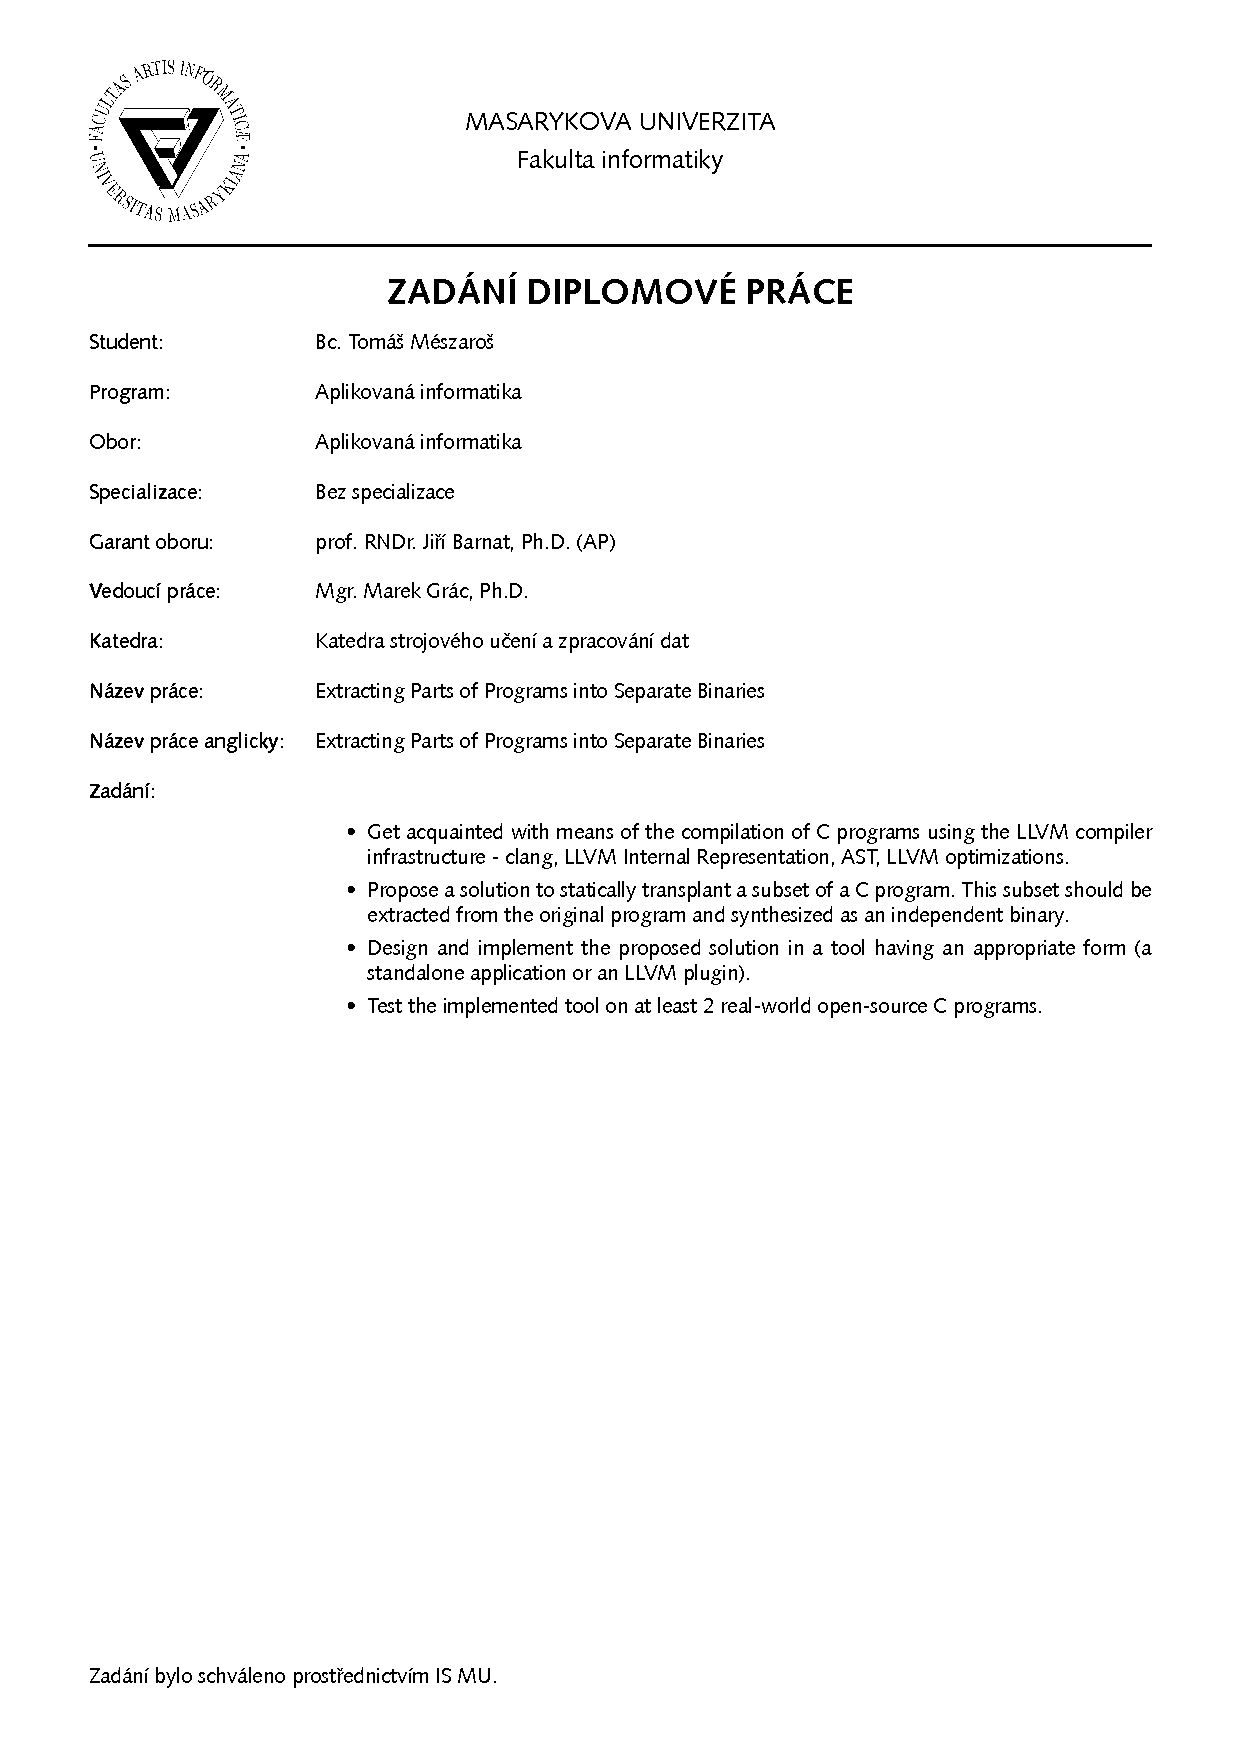
\includepdf[pages=-]{zadanie.pdf}

\includepdf[pages=-]{blank.pdf}

\includepdf[pages=-]{prehlasenie.pdf}

\begin{ThesisDeclaration}
    \DeclarationText
    \AdvisorName
\end{ThesisDeclaration}

\begin{ThesisThanks}
I would like to thank my advisor Marek Grác for his time and for making this
thesis possible.
Many thanks to my consultant Viktor Malík for sharing his knowledge and
willingness to always help.
Thanks to Pavel Odvody for coming up with the thesis idea and for his
valuable feedback.

A big thanks to my family, Alena, Ľudovít and Martin for their support
during my studies.

I would like to thank everybody that supported me in any shape or form on this
journey. In no particular order: Majo, Jozef, Paťo, Mikasa, Astrix,
Miša, Markéta, Tomáš, Marcel, Janka, Hanka, Žofka, Vlastík, Mišo, Dominik,
Stela, Ondra, Kristína, Grandma, Lukáš, Majky, Maroš, Palo and others that I
forgot to mention. Thank you.
\end{ThesisThanks}

\begin{ThesisAbstract}
This thesis presents method for extracting parts of programs into separate
binaries.
The extraction method is based on static analysis of the program source code
and leverages the LLVM infrastructure.
Solution is implemented as LLVM optimization pass and is integrated into the
open-source tool APEX.
Extracted binary can be executed repeatedly without any other intermediary
manual steps.
Final solution is tested on three UNIX utilities.

%Táto práca prezentuje metódu na extrakciu časti programu do separátnych
%binárnych súborov.
%Metóda extrakcie je založená na statickej analýze zdrojového kódu a využíva LLVM
%infraštruktúru.
%Riešenie je implementované ako LLVM optimalizačný priechod a následne integrované
%do open-source nástroja APEX.
%Extrahovaný binárny súbor môže byť opakovane spúšťaný bez ďalších manuálnych
%medzikrokov.
%Finálne riešenie je testované na troch UNIXových nástrojoch.
\end{ThesisAbstract}

\begin{ThesisKeyWords}
static analysis, program analysis, program extraction, intermediate
representation, code optimization, LLVM
\end{ThesisKeyWords}

\MainMatter
\tableofcontents



% === CHAPTER ==================================================================
\chapter{Introduction}
\label{chap:intro}

Running debugger with set breakpoint at the selected variable location is the
usual approach when user wants to know value of the variable.
Unfortunately, this approach is cumbersome when user wants to execute this
procedure many times.
It consists of many manual steps, which are time consuming to perform.
Ideally, there should be a script that accepts line of code as an input and
produces value of the selected variable once the execution hits the desired
line of code.

Normally, this method would require to use debugger with the scripting support
and write scripts that would instruct debugger what exactly to do, basically
replicating the manual approach.

Instead of scripting debugger to do the extraction, we could write a tool that
would accept line of code as an input, run analysis on where the execution
path in the program occurs to get to the target instruction and transplant
subset of the program with computed execution path into the separate binary.
This way, user would have separate executable that, when executed, would produce
value of the targeted instruction without having to manually step thought or
script debugger.

This thesis aims to devise method for statically transplanting a subset of a C
program and implement it in a open-source tool.
The selected program subset should be extracted from the
original program provided by the user and synthesized as an independent,
executable binary.

Proposed solution should be implemented in a tool having appropriate form,
preferably using LLVM infrastructure. It should be user friendly and allow user
to provide input of choice.

Implemented tool should be tested on at least two real-world open-source C
programs in order to find where the room for improvements is and what could be
achieved in the future.

% summary of the thesis

The remainder of this thesis is structured as follows.

In \autoref{chap:llvm} we briefly introduce the LLVM compiler
infrastructure and explain what makes it so popular.

We present method that is able to extract part of programs in
\autoref{chap:design}, while \autoref{chap:implementation} explains specific
implementation details.

Experiments and results are discussed in the chapter
\autoref{chap:experiments}.

Finally, \autoref{chap:conclusions} summarizes the results of this thesis and
presents possible further research and development opportunities.


% === CHAPTER: LLVM ============================================================
\chapter{The LLVM Compiler Infrastructure:}
\label{chap:llvm}

\emph{The LLVM project is a collection of modular and reusable compiler and
toolchain technologies.} \cite{llvm}
Designed to be compatible with already existing UNIX tools, LLVM includes
set of low-level tools like Clang compiler, assembler, debugger, etc. \cite{asoa}


\section{Architecture}
\label{sec:llvm-arch}

The main distinguishing feature that separates LLVM from other compiler
frameworks is its internal structure. LLVM compiler leverages tree-phase
architecture shown in the \autoref{fig:llvm_arch} to achieve higher degree of
flexibility and modularity.

\begin{figure}[ht]
    \centering
    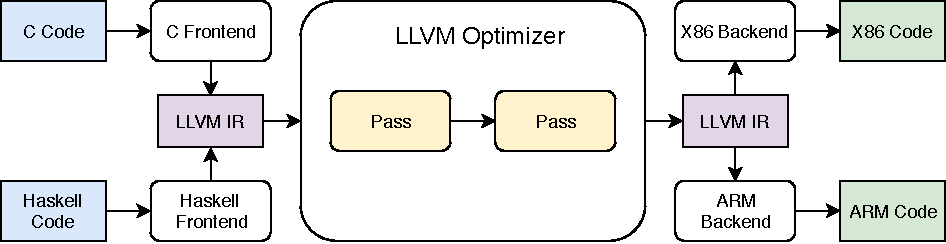
\includegraphics[]{images/llvm/llvm_arch.pdf}
    \caption{LLVM Compiler Architecture.}
    \label{fig:llvm_arch}
\end{figure}

\begin{myItemize}
\item Frontend is responsible for the first phase of compilation. Input code is
parsed, processed, validated for errors and translated into the LLVM Intermediate
Representation (IR). IR is used to represent code in the compiler (more about IR
in \autoref{sec:llvm-ir}).
\item IR code may be optionally put through
optimization during the second phase. Optimizer can use various analysis and transform
passes to improve the code and emit modified IR.
\item Third and final phase is the code generation. Various backends take
IR and produce platform specific machine code.
\end{myItemize}

The huge advantage of this architecture is the fact that the optimizer and
backend phase work with the IR instead of the language specific source code.
This means that the compiler developer can write frontend for the new language
that translates source code to the IR and does not have to write optimizations
and code generator because LLVM infrastructure works with the IR and already
provides those facilities.

\section{Intermediate Representation}
\label{sec:llvm-ir}

LLVM assembly language is a Static Single Assignment (SSA)
\footnote{
SSA means that each variable is defined before it is being used and is assigned
exactly once.
}

based
representation that provides type safety, low-level operations, flexibility,
and the capability of representing ‘all’ high-level languages cleanly. It is
the common code representation used throughout all phases of the LLVM
compilation strategy.
\cite{llvm-ir}

LLVM code can be represented by the following three equivalent forms:
\begin{myEnumerate}
\item Compiler intermediate representation (IR) that resides in the memory.
\item Bitcode stored in the file.
\item Assembly representation that is human readable.
\end{myEnumerate}

\bigskip
\noindent
We present the simple C function foo, stored in the file foo.c:

\begin{minted}[label=foo.c,frame=lines,framesep=10pt]{C}
int foo(int a, int b) {
    if (a > b) {
        return a+b;
    } else {
        return a-b;
    }
}
\end{minted}

The LLVM Intermediate Representation of the foo.c is available in the following
code:

\begin{minted}[label=foo.s,frame=lines,framesep=10pt]{llvm}
define i32 @foo(i32 %a, i32 %b) #0 {
entry:
  %retval = alloca i32, align 4
  %a.addr = alloca i32, align 4
  %b.addr = alloca i32, align 4
  store i32 %a, i32* %a.addr, align 4
  store i32 %b, i32* %b.addr, align 4
  %0 = load i32, i32* %a.addr, align 4
  %1 = load i32, i32* %b.addr, align 4
  %cmp = icmp sgt i32 %0, %1
  br i1 %cmp, label %if.then, label %if.else

if.then:                                          ; preds = %entry
  %2 = load i32, i32* %a.addr, align 4
  %3 = load i32, i32* %b.addr, align 4
  %add = add nsw i32 %2, %3
  store i32 %add, i32* %retval, align 4
  br label %return

if.else:                                          ; preds = %entry
  %4 = load i32, i32* %a.addr, align 4
  %5 = load i32, i32* %b.addr, align 4
  %sub = sub nsw i32 %4, %5
  store i32 %sub, i32* %retval, align 4
  br label %return

return:                                           ; preds = %if.else, %if.then
  %6 = load i32, i32* %retval, align 4
  ret i32 %6
}
\end{minted}

LLVM programs are composed from units called \textbf{modules}. Two or more
modules can be combined together with the linker.\footnote{
Two bitcode modules can be linked with tool llvm-link. More info at
\url{https://llvm.org/docs/CommandGuide/llvm-link.html}
}
\autoref{fig:llvm_module} shows architecture of the LLVM module.

\begin{figure}[ht]
    \centering
    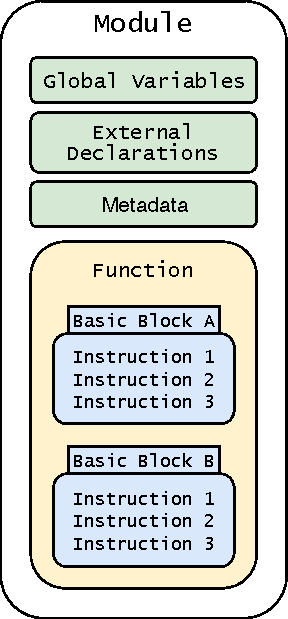
\includegraphics[]{images/llvm/llvm_module.pdf}
    \caption{LLVM Module Structure.}
    \label{fig:llvm_module}
\end{figure}

Each module can include several functions, which in turn can contain several
basic blocks.

\textbf{Function} in the LLVM defines a list of basic blocks, which form the
control flow graph of the function (blocks A and B in \autoref{fig:llvm_module}).
\cite{llvm-ir}

A \textbf{basic block} is a type of a container that contains instructions that
are executed sequentially.\cite{llvm-bb} Each basic blocks is formed with
non-terminating instructions and single terminator instruction at the end of
the block. Only terminator instructions can terminate a basic block\footnote{
\url{https://llvm.org/doxygen/classllvm_1_1TerminatorInst.html}
}
(in the case of \autoref{fig:llvm_module}, terminators would be Instruction 3
in both basics blocks).

In the case of foo.s, we can see that the function foo contains four basic
blocks: entry, if.then, if.else and return.
Basic block entry is special in a way that it is the first basic block in the
foo function and thus is executed always first. entry basic block is also
prohibited to have any predecessors unlike for example if.then, which have
entry as it processor and thus allow branching of the program.

\section{Optimizations}
\label{sec:llvm-opt}

LLVM uses the concept of passes for the optimizations. Concrete optimizations
are implemented in a \textbf{pass} that works with some portion of program code
(e.g.  module, function, loop, etc.) to collect or transform portion of
the code.
\cite{llvm-passes} Pass is a optimization unit that is executed in the second
phase of the compilation process (\autoref{fig:llvm_arch}) or can be executed
separately with opt tool.\footnote{
\url{https://llvm.org/docs/CommandGuide/opt.html}
}

There are three types of passes:

\begin{myEnumerate}
\item \textbf{Analysis:} Collect information from the IR and feed it into
the other passes. They can be also used for the debugging purposes (e.g.
pass that counts number of functions in the module).

Examples:
\begin{myItemize}
\item basiccg: Basic CallGraph Construction.
\item dot-callgraph: Print Call Graph to “dot” file.
\item instcount: Counts the various types of Instructions.
\end{myItemize}

\item \textbf{Transform:} Change the program in some way. They can use
data that was produced by analysis pass.

Examples:
\begin{myItemize}
\item dce: Dead Code Elimination.
\item loop-deletion: Delete dead loops.
\item loop-unroll: Unroll loops.
\end{myItemize}

\item \textbf{Utility:} Do not fit into analysis or transform pass categories.

Examples:
\begin{myItemize}
\item verify: Module Verifier.
\item view-cfg: View CFG of function.
\item instnamer: Assign names to anonymous instructions.
\end{myItemize}

\end{myEnumerate}


% === SECTION: Clang ===========================================================
\section{Clang}
\label{sec:llvm-clang}

\emph{The Clang project provides a language front-end and tooling
infrastructure for languages in the C language family.}\cite{clang}

Clang compiler uses LLVM infrastructure for optimizations and code generation
(as is described in \autoref{fig:llvm_arch}).
Clang AST (Abstract Syntax Tree)\footnote{
Syntactic structure of the source code represented in as a tree.
} closely represents the underlying code and does not abstract away elements
that are useful refactoring tools.\cite{clang-ast}.

\begin{minted}[label=add.c,frame=lines,framesep=10pt]{C}
int add(int a, int b) {
    return a+b;
}
\end{minted}

Getting the AST from the code above is as simple as running clang with the
following command line arguments:

\mintinline{text}{
clang -Xclang -ast-dump -fsyntax-only add.c
}

\begin{minted}[label=add.c AST,frame=lines,framesep=10pt,breaklines]{text}
TranslationUnitDecl 0x622b600 <<invalid sloc>> <invalid sloc>
... leaving out internal clang declarations ...
`-FunctionDecl 0x6280fa8 <ast.c:1:1, line:3:1> line:1:5 add 'int (int, int)'
  |-ParmVarDecl 0x622c268 <col:9, col:13> col:13 used a 'int'
  |-ParmVarDecl 0x6280ed0 <col:16, col:20> col:20 used b 'int'
  `-CompoundStmt 0x6281150 <col:23, line:3:1>
    `-ReturnStmt 0x6281138 <line:2:2, col:11>
      `-BinaryOperator 0x6281110 <col:9, col:11> 'int' '+'
        |-ImplicitCastExpr 0x62810e0 <col:9> 'int' <LValueToRValue>
        | `-DeclRefExpr 0x6281090 <col:9> 'int' lvalue ParmVar 0x622c268 'a' 'int'
        `-ImplicitCastExpr 0x62810f8 <col:11> 'int' <LValueToRValue>
          `-DeclRefExpr 0x62810b8 <col:11> 'int' lvalue ParmVar 0x6280ed0 'b' 'int'
\end{minted}

Clang AST provides great value for developers. Nevertheless, instead of the
AST, we will work in this thesis directly with the IR because it provides
greater flexibility via LLVM API.\footnote{
\url{https://llvm.org/doxygen/namespacellvm.html}
}

Clang also is able to emit IR for the add.c with the following command:

\mintinline{text}{
clang -S -emit-llvm ast.c -o ast.s
}

\begin{minted}[label=add.s,frame=lines,framesep=10pt,breaklines]{llvm}
define i32 @add(i32 %a, i32 %b) #0 {
entry:
  %a.addr = alloca i32, align 4
  %b.addr = alloca i32, align 4
  store i32 %a, i32* %a.addr, align 4
  store i32 %b, i32* %b.addr, align 4
  %0 = load i32, i32* %a.addr, align 4
  %1 = load i32, i32* %b.addr, align 4
  %add = add nsw i32 %0, %1
  ret i32 %add
}
\end{minted}


% ==============================================================================
% === CHAPTER: Design of the Method ============================================
\chapter{Extracting Program Subsets}
\label{chap:design}

In this chapter, we introduce the method for extracting parts of programs
from the provided user input.

Starting with the method overview in the \autoref{sec:method_overview} where we
define what is the user input and briefly outline the method itself, what it
does and what are the steps for achieving the final result.

We follow with the example of the method from the user perspective in the
\autoref{sec:method_example}.

After example, we present in detail each major step that is followed.
Starting with computing data dependencies graph
(\autoref{sec:design-dep}).
Following with the procedure for finding connected components in the computed
data dependencies graph (\autoref{sec:design-components}).
Next follows introduction of the call graph (\autoref{sec:design-callgraph}) and
subsequently procedure for finding path from source to target in it
(\autoref{sec:design-path}).
The chapter ends with the section describing methods on eliminating dead
components and functions from the code (\autoref{sec:design-removing}).


% ===== SECTION: Method Overview ===============================================
\section{Method Overview}
\label{sec:method_overview}

% method input definition
Mandatory \textbf{input} for the method is a touple with the following
definition:

$$
input \equiv (code, target)
$$

where:
\begin{myItemize}
\item \textbf{code} is a C program source code compiled into the llvm bitcode.
\item \textbf{target} is an integer value representing line of code from the
C program source code.
\end{myItemize}

We also define \textbf{source} as an entry to the C program
(\mintinline{text}{main} function).

% what the method does

The method determines what parts of the \emph{input} to extract according to
the \emph{source} and \emph{target}.
Procedure subsequently calculates possible execution path up to the
\emph{target} and extracts this execution path into the separate, functioning
executable.

Barring implementation specific details (which are discussed in the
\autoref{chap:implementation}), the method can be summarized by the following
five steps:

\begin{myEnumerate}
\item Compute data dependencies between instructions.
\item Find connected components in the computed data dependencies inside
every function.
\item Construct call graph, mapping between connected components and functions
that are being called from these components.
\item Find path from source to target in the call graph.
\item Eliminate dead components and functions that do not depend on the path.
\end{myEnumerate}

% what is the result of the method
Upon completion of the steps mentioned above, the llvm bitcode is produced as
an \emph{output}.
We can define \textbf{output} as the extracted part of the original program
according to the \emph{source} and \emph{target} while keeping the consistency
of the code intact.
By \textbf{consistency}, we mean that the \emph{output} code is in a such state
that it was possible to be compiled.
\emph{Output} is expected to be runnable the same way as
the original.
\textbf{**TODO? explain more here or in another chapter what it means for IR to
be compiled without problems?**}

% === SECTION: Method Example ==================================================
\section{Example}
\label{sec:method_example}

User provided us with the \emph{input} in the form of the following
C program source code that is stored in the file \mintinline{text}{example.c}:

\begin{minted}[label=example.c,frame=lines,framesep=10pt,linenos]{C}
int foo(int n) {
    int x = n + 10;
    return x;
}

int bar(void) {
    int y = 42;
    return y;
}

int main(void) {
    int some_int = 10;
    int foo_result = foo(some_int);
    int bar_result = bar();
    return 0;
}
\end{minted}

Since our method does not work directly with the C source code but instead
works with the LLVM Intermediate Representation (IR), lets use clang and emit
IR from the presented C source code in order to demonstrate the procedure more
clearly:
\footnote {
Flag \mintinline{text}{-S} tells clang to only run preprocess and
compilation steps, while \mintinline{text}{-emit-llvm} makes sure to use the LLVM
representation for assembler and object files. For detailed description of
various clang flags, visit
\url{https://clang.llvm.org/docs/ClangCommandLineReference.html}.
}

\begin{minted}[frame=lines,framesep=10pt]{bash}
  clang -S -emit-llvm example.c -o example.s
\end{minted}

Emitted LLVM IR is stored in the file \mintinline{text}{example.s} and
has the following structure:\footnote{
Strictly speaking, this is not exactly the IR code that would be emitted by the
clang. We have stripped it out of the module info and comments to make it more
readable. To see the unmodified \mintinline{text}{example.s}, please go to the
\autoref{appendix:example}.
}

\begin{minted}[label=example.s,frame=lines,framesep=10pt,linenos]{llvm}
define i32 @foo(i32 %n) #0 {
entry:
  %n.addr = alloca i32, align 4
  %x = alloca i32, align 4
  store i32 %n, i32* %n.addr, align 4
  %0 = load i32, i32* %n.addr, align 4
  %add = add nsw i32 %0, 10
  store i32 %add, i32* %x, align 4
  %1 = load i32, i32* %x, align 4
  ret i32 %1
}

define i32 @bar() #0 {
entry:
  %y = alloca i32, align 4
  store i32 42, i32* %y, align 4
  %0 = load i32, i32* %y, align 4
  ret i32 %0
}

define i32 @main() #0 {
entry:
  %retval = alloca i32, align 4
  %some_int = alloca i32, align 4
  %foo_result = alloca i32, align 4
  %bar_result = alloca i32, align 4
  store i32 0, i32* %retval, align 4
  store i32 10, i32* %some_int, align 4
  %0 = load i32, i32* %some_int, align 4
  %call = call i32 @foo(i32 %0)
  store i32 %call, i32* %foo_result, align 4
  %call1 = call i32 @bar()
  store i32 %call1, i32* %bar_result, align 4
  ret i32 0
}
\end{minted}

% next point
User also provided the line number \textbf{7} from the
\mintinline{text}{example.c} as the target, which corresponds to the line
\textbf{16} from the \mintinline{text}{example.s}. Source is the main function.

Procedure for finding mapping between C code referenced by the user input and
its analogous IR instruction is implementation detail and is be described
in the \autoref{chap:implementation}.

% next point
When we apply the method on the contents of the
\mintinline{text}{example.s} with respect to the source and target,
we get the result stored in the file
\mintinline{text}{example_extracted.s} with the following code:

\begin{minted}[label=example\_extracted.s,frame=lines,framesep=10pt]{llvm}
define i32 @bar() #0 {
entry:
  %y = alloca i32, align 4
  store i32 42, i32* %y, align 4
  ret i32 %0
}

define i32 @main() #0 {
entry:
  %bar_result = alloca i32, align 4
  %call1 = call i32 @bar()
  store i32 %call1, i32* %bar_result, align 4
  ret i32 0
}
\end{minted}

As we can see from the \mintinline{text}{example.c}, execution path from
the program entry in the \mintinline{text}{main} function (which we will
call \textbf{source}) to the \textbf{target} does not include function
\mintinline{text}{foo} and its associated instructions, they can be removed.
We are left only with function \mintinline{text}{bar} which contains target,
and necessary instructions in the function \mintinline{text}{main} along with
the \mintinline{text}{main} itself.
\\
\\
We can now take \mintinline{text}{example_extracted.s} and recompile it back
into the functioning executable.\footnote{
More about recompilation in the \autoref{chap:implementation}.
}


% === SECTION: Computing Data Dependencies =====================================
\section{Computing Data Dependencies}
\label{sec:design-dep}

% motivation
In order to identify what parts of the IR we can afford to remove, it is
imperative to compute dependencies between instructions.
When removing instructions, we need to preserve consistency of the remaining
code so that it can be later compiled into a functional executable.
To ensure this, we first compute dependencies among instructions.

% definitions
We recognize two types of dependencies between IR instructions: control and data
dependencies.
The following terminology and procedures for computing dependencies that we use
are due to the Marek Chalupa master's thesis \textit{Slicing of LLVM Bitcode}
\cite{dg}.

\begin{myItemize}
\item ``\textbf{Control dependence} explicitly states what nodes are
controlled by which predicate.``
\item ``A \textbf{data dependence} edge is between nodes n and
m iff n defines a variable that m uses and there is no intervening definition
of that variable on some path between n and m. In other words, the definitions
from n reach uses in m.``
\end{myItemize}

% method
The crucial information comes from data dependencies. We need to make sure that
the IR integrity will remain intact after we are done with removing IR
instructions.

The following example demonstrates data dependencies for the
previously presented \mintinline{text}{example.c} source code.
Taking closer look specifically at the function \mintinline{text}{main}:

\begin{minted}[frame=lines,framesep=10pt]{llvm}
define i32 @main() #0 {
entry:
  %retval = alloca i32, align 4
  %some_int = alloca i32, align 4
  %foo_result = alloca i32, align 4
  %bar_result = alloca i32, align 4
  store i32 0, i32* %retval, align 4
  store i32 10, i32* %some_int, align 4
  %0 = load i32, i32* %some_int, align 4
  %call = call i32 @foo(i32 %0)
  store i32 %call, i32* %foo_result, align 4
  %call1 = call i32 @bar()
  store i32 %call1, i32* %bar_result, align 4
  ret i32 0
}
\end{minted}

Taking \mintinline{text}{main} code, we can construct graph G where V is set
of vertices (in our case vertex is instruction) and E is set of edges (in our
case, edge between vertices V1 and V2 represents data dependency between
instruction V1 and V2).
In order to compute data dependencies, we use \mintinline{text}{dg} library.
\cite{dg}
\footnote{
For more info please visit \url{https://github.com/mchalupa/dg} \cite{dg}.
We will take a closer look at \mintinline{text}{dg} in the
\autoref{chap:implementation}.
}

Computed \textbf{data dependency graph} for instructions from the function
\mintinline{text}{main} is presented in the \autoref{fig:data_deps_graph}.
This graph is stored and used in the next step of the method for finding
connected components (\autoref{sec:design-components}).

\begin{figure}[ht]
    \centering
    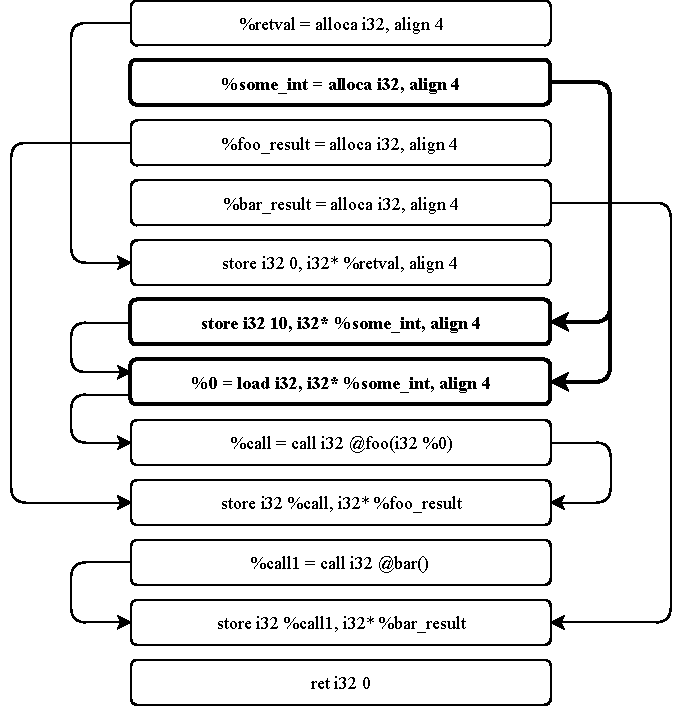
\includegraphics[]{images/main_dependencies.pdf}
    \caption{Data dependencies graph of the \mintinline{text}{main} function instructions.}
    \label{fig:data_deps_graph}
\end{figure}

Taking a closer look at the instruction:
\mintinline{llvm}{%some_int = alloca i32, align 4}.
We see that the following instructions have data dependency on the
\mintinline{llvm}{%some_int}

\begin{minted}[frame=lines,framesep=10pt, escapeinside=||]{llvm}
  store i32 10, i32* %some_int, align 4
  %0 = load i32, i32* %some_int, align 4
\end{minted}

It is apparent that both instructions need \mintinline{llvm}{%some_int} for
their operand. If we removed
\mintinline{llvm}{%some_int = alloca i32, align 4}
without taking into consideration that there are two
instructions that depend on it, we would get into inconsistent state and two
dependent instructions would contain undefined values as their operand.\footnote{
More about undefined values at
\url{https://llvm.org/docs/LangRef.html\#undefined-values},
\url{https://llvm.org/docs/FAQ.html\#what-is-this-undef-thing-that-shows-up-in-my-code},
\url{https://llvm.org/doxygen/classllvm_1_1UndefValue.html}
}
This would lead into unsuccessful recompilation of the modified code back into
the executable.

% === SECTION: Finding Connected Components ====================================
\section{Finding Connected Components}
\label{sec:design-components}

% motivation
Having shown in the previous section what are inter-instruction data
dependencies and how important they are in relation to the code consistency.
However, they do not fully solve our problem of knowing when it is safe to
remove instruction.
Data dependencies between only two instructions do not reveal the whole picture.
Since we have computed and stored graph of data dependencies, let us propose the
idea of computing connected components of this graph.

% definitions

We define \textbf{connected component} as an isolated subgraph, where
each pair of vertices is connected by some path.

We use \textbf{data dependency graph} computed in the section
\autoref{sec:design-dep} to find its connected components by using the following
algorithm:

\begin{minted}[label=finding components,escapeinside=||,frame=lines,framesep=10pt]{text}
0. Let G = data dependency graph
1. Run |Breadth-first search \cite{clrs}| on G to visit each instruction
2. IF instruction not in any component:
      Create new component and put instruction inside
   ELSE:
      Go to next instruction
\end{minted}

Running the above mentioned algorithm on the \textbf{data dependency graph}
produces connected components for each function in the input.
As an example, we present components for the \mintinline{text}{main} function
in the \autoref{fig:connected_components_graph} (for the clarity, each component
has its own color).

\begin{figure}[ht]
    \centering
    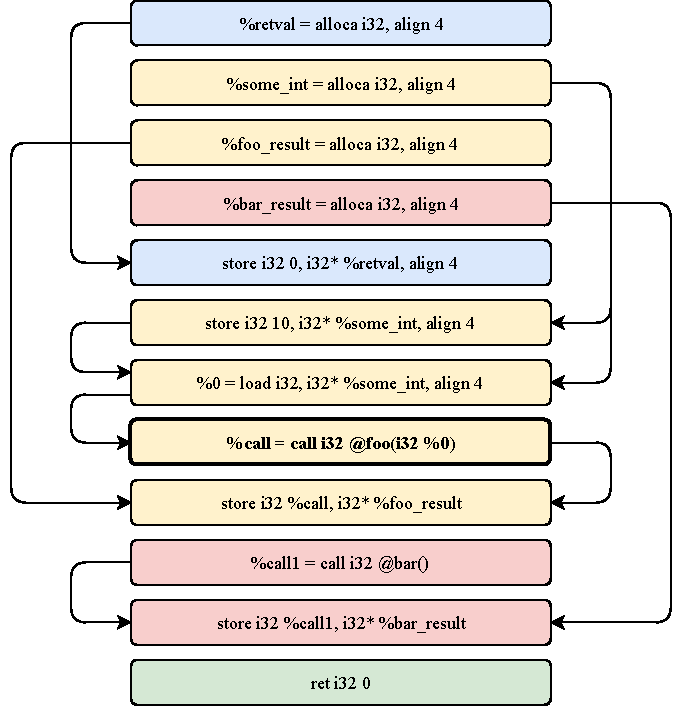
\includegraphics[]{images/main_components.pdf}
    \caption{Connected components of the data dependencies graph
    for the \mintinline{text}{main} function instructions. Individual components
    are differentiated by the color.}
    \label{fig:connected_components_graph}
\end{figure}

% why having components is good

Having instructions within each function separated into connected components
comes useful especially because we can answer the question if some particular
instruction is in data dependency relationship with multiple other instructions
(instructions that form a data dependency path, etc.).

% === SECTION: Computing Call Graph ============================================
\section{Computing Call Graph}
\label{sec:design-callgraph}

%motivation

In respect to the program execution flow, user provided the target and we know
the source.
In order to proceed further, it is needed to compute possible paths from
source to target that could be used by the execution of the program.
Computing and walking the call graph of the program can produce for us this
piece of information.

% definition

A \textbf{call graph}\footnote{
More technically, \emph{call multigraph} \cite{data_flow}.}
is a control flow graph that represents relationship
between program procedures in respect to control flow.\cite{data_flow}
Having call graph $G = \{V, E\}$, set of vertices $V$ typically represents
functions and set of edges $E$ represents transfer of control flow from one
function to another.

In our context, call graph represents relationship between individual
connected components (computed in the \autoref{sec:design-components})
and functions that are being called from these components by one of its
instructions. In other words, our call graph is a set of mappings from
components to the function (or functions).


% example

We construct the call graph using the following algorithm:

\begin{minted}[label=computing call graph,escapeinside=||,frame=lines,framesep=10pt]{text}
0. Let FS = set of functions in the code
1. Let CS(f) = set of components inside function f
2. FOR EACH function F in the set FS:
      FOR EACH component C in the set CS(F):
         FOR EACH instruction I in the component C:
            IF instruction I is a call instruction to some function X:
                Store information X gets called from the C
\end{minted}

Running the presented algorithm on the \textbf{data dependence graph}
of the \mintinline{text}{main} function that we computed earlier
(\autoref{fig:connected_components_graph}) produce call graph structure
shown in the \autoref{fig:call_graph}. We know that in the context of the
\mintinline{text}{main} function, there are four distinct components.
We can see from the computed call graph, that
\mintinline{llvm}{i32 @foo(i32 %n)} is being called from the
\emph{yellow} component, and
\mintinline{llvm}{i32 @bar()} is being called from the \emph{red} component.

\begin{figure}[ht]
    \centering
    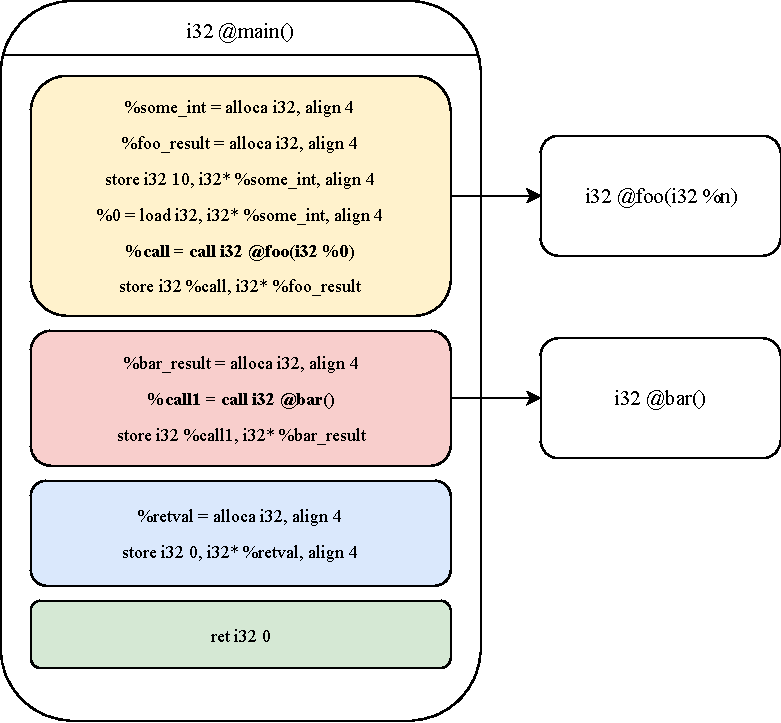
\includegraphics[]{images/main_callgraph.pdf}
    \caption{Call graph computed from the connected components
    as shown in the \autoref{fig:connected_components_graph}.}
    \label{fig:call_graph}
\end{figure}


% === SECTION: Finding Path ====================================================
\section{Finding Path from Source to Target}
\label{sec:design-path}

% motivation

Having call graph represented in the structure shown in the
\autoref{fig:call_graph} is beneficial for finding program execution flow path
between specific components within the program in relation to their
dependencies. We can find path from source to target and know which components
this path contains.

% definitions

\emph{''A \textbf{path} is a simple graph whose vertices can be arranged in a linear sequence in
such a way that two vertices are adjacent if they are consecutive in the sequence,
and are nonadjacent otherwise.''}\cite{graph_theory} In our case, linear
sequence of vertices consists of components computed in the
\autoref{sec:design-components}.

% method

The reason why we constructed call graph in the previous chapter is now apparent.
We want to find a path from source to the target and in doing so, know which
connected components are part of this path or not.
Potentially, there may exist infinite number of such paths. From
the optimization standpoint, it would be fitting to find all (or at least as
many as we can) paths and pick some path according to selected optimization
criteria (shortest path, path with smallest connected components, etc.).
However, for our purposes, it will be sufficient to find any path, because
our method does not try to optimize final code in respect to size, speed, etc.

We will use the following algorithm in order to find a path from source to target
in the call graph:

\begin{minted}[label=finding path,escapeinside=||,frame=lines,framesep=10pt]{text}
0. Let G = call graph
1. Run Breadth-first search on G to find path from source to target
\end{minted}

\begin{figure}[ht]
    \centering
    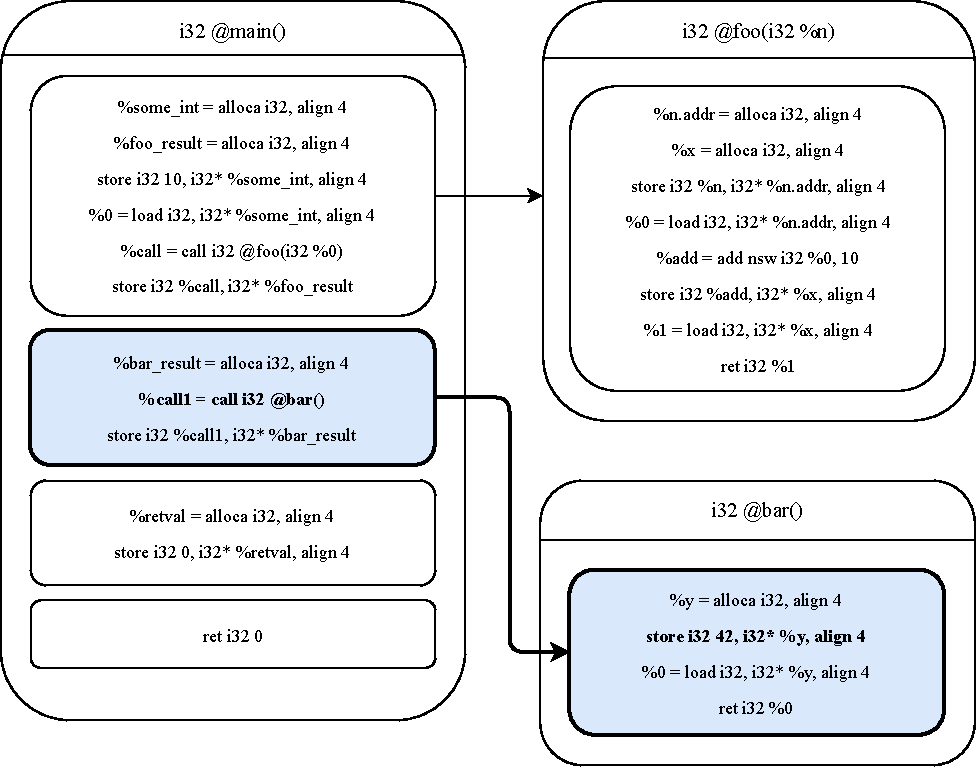
\includegraphics[]{images/main_path.pdf}
    \caption{Path from \textbf{source} to \textbf{target} computed on the
    \autoref{fig:call_graph}. Components in the path are \emph{blue}.
    }
    \label{fig:path}
\end{figure}

Given the source and target, we can see from the \autoref{fig:path} that path
only contains two components, one from \mintinline{text}{main} function and
another from \mintinline{text}{bar}. These two components are going to be the
core of the final, extracted program.

% === SECTION: Eliminating Dead Code ===========================================
\section{Eliminating Dead Components and Functions}
\label{sec:design-removing}

% motivation
The final step of our method is extraction of the desired parts of code.
We do this by eliminating so-called dead components and functions.

% definition
An element of the code is defined as \textbf{dead} if and only if its removal
does not break reachability of target from source and integrity of the code.

In other words, we can safely remove dead elements from the code without being
worried that the remaining code cannot be compiled and that the execution
starting from source will not reach target.

In the previous section, we described how to find a path from source to target.
Since this path should be perserved, each component that is a part of the path
cannot be marked as dead.
Therefore, components outside of the path have to be explored and the decision
must be made whether they can be marked as dead or not.

We  use the following basic algorithm for finding and eliminating dead
components:

\begin{minted}[label=eliminating dead components,escapeinside=||,frame=lines,framesep=10pt]{text}
0. Let CS = set of all components in the code
1. Let PATH = set of components on the path from source to target
2. FOR EACH component C in set CS:
      IF component C is not in the set PATH:
         IF component C does not contain terminator:
             Mark component C as DEAD
3. Remove all components marked as DEAD
\end{minted}

% example

After applying the presented algorithm for eliminating dead components on the
code from \mintinline{text}{example.s} we get the result that is shown
in \autoref{fig:removing_prepare}.
Components marked as dead are colored \emph{red} because they are not
a part of the path.
The \emph{yellow} component with the single instruction stands out.
This component is not marked as dead and will not be removed because it contains
a terminator instruction \mintinline{llvm}{ret i32 0}.\footnote{
\url{https://llvm.org/doxygen/classllvm_1_1TerminatorInst.html}
More about terminators and why they need special treatment in the
\autoref{chap:implementation}.
}
Finally, all components marked as dead are removed and we are left with the
code that we presented in \autoref{sec:method_example}
(\mintinline{text}{example_extracted.s}).
Call graph of the \mintinline{text}{example_extracted.s} is visualized in
\autoref{fig:removing_done}.

\begin{figure}[ht]
    \centering
    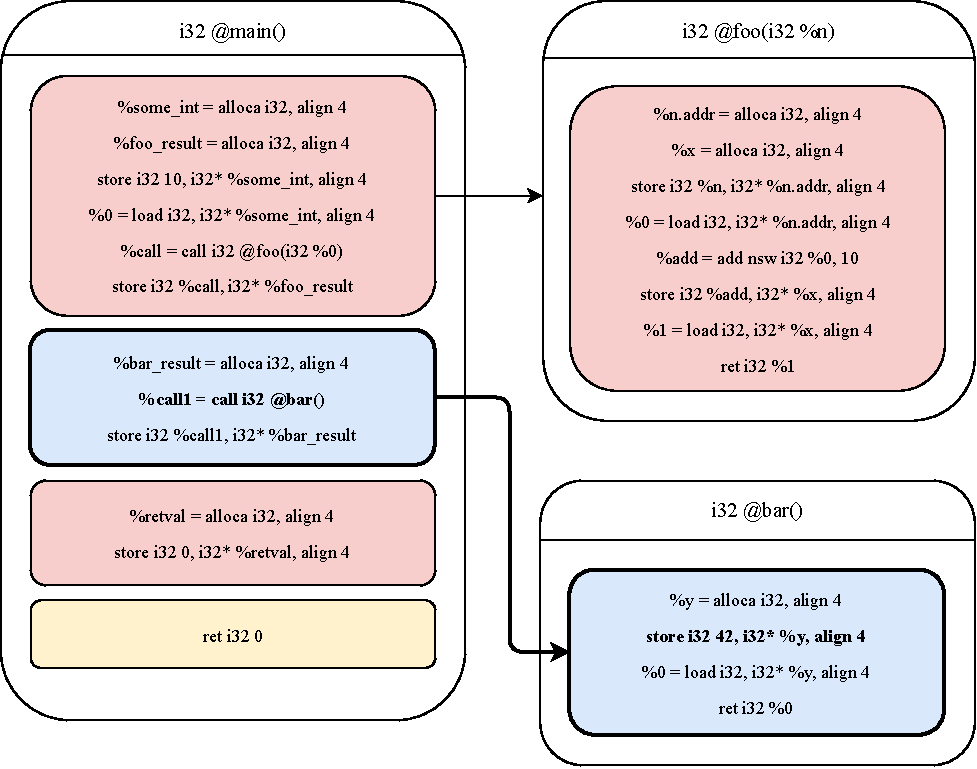
\includegraphics[]{images/main_removing_prepare.pdf}
    \caption{
    \mintinline{text}{example.s}:
    Components selected for removal are marked \emph{red}.
    \emph{Yellow} component is not marked for removal, because it contains a
    terminator instruction.
    }
    \label{fig:removing_prepare}
\end{figure}

\begin{figure}[ht]
    \centering
    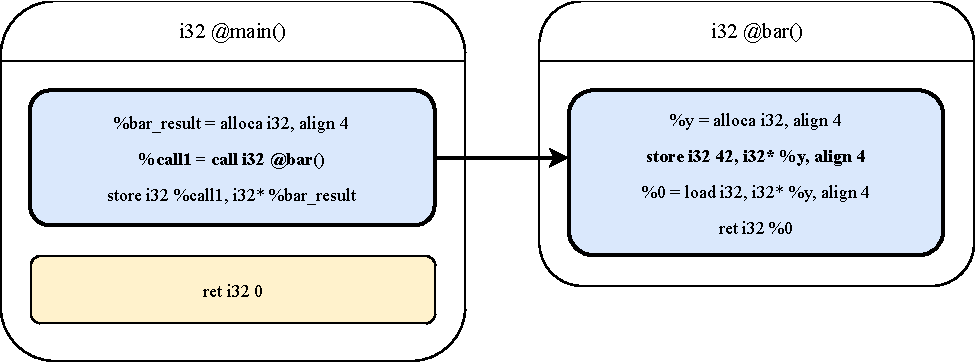
\includegraphics[]{images/main_removing_done.pdf}
    \caption{
    \mintinline{text}{example_extracted.s}:
    Final state after removing dead components and functions.
    \mintinline{text}{example.s}.
    }
    \label{fig:removing_done}
\end{figure}

% conclusion

Unfortunately, the basic algorithm presented above only works correctly with
non-complex inputs such as the one in \mintinline{text}{example.s}.

We present two extensions of the \mintinline{text}{example.s} program along with
improvements of the basic algorithm that help to handle these extensions.

\clearpage

% === SUB-SECTION: External Function ===========================================
\subsection{Path Depending on the External Function}
\label{subsec:path_function}

The first problem is that there may exist a function that is not part of the
path but that is called by one instruction on the path.
In such case, when looking upon \autoref{fig:mod1_prepare}, we see that
function bar calls function qux, but qux is not part of the computed path (only
components with the blue color are part of the path, that is one component from
main and one from foo).
This is problematic for the basic algorithm that we introduced in the
\autoref{sec:design-removing}.
This basic algorithm would mark qux as dead and subsequently remove this
function. However, this would break code integrity, because function qux has to
be called in order for the execution to correctly proceed.
Therefore, we propose modified algorithm for eliminating dead components that
will take into the account the above described possibility.

\begin{minted}[label=eliminating dead components - mod1,escapeinside=||,frame=lines,framesep=10pt]{text}
0. Let CS = set of all components in the code
1. Let PATH = set of components on the path from source to target
2. Recursively find all called functions that originate from PATH
   using Breath-first search and add them to the PATH.
3. FOR EACH component C in set CS:
      IF component C is not in the set PATH:
         IF component C does not contain terminator:
             Mark component C as DEAD
4. Remove all components marked as DEAD
\end{minted}


We modify the \mintinline{text}{example.c} by introducing a new function
\mintinline{C}{int qux(void)}. Also, we change line 7 of the
\mintinline{text}{example.c} from
\mintinline{C}{int y = 42} to \mintinline{C}{int y = qux()}, the resulting code
is shown in \mintinline{text}{example_mod1.c}:

% mod1 C code
\begin{minted}[label=example\_mod1.c,frame=lines,framesep=10pt,linenos]{C}
int foo(int n) {
    int x = n + 10;
    return x;
}

int qux(void) {
    return 42;
}

int bar(void) {
    int y = qux();
    return y;
}

int main(void) {
    int some_int = 10;
    int foo_result = foo(some_int);
    int bar_result = bar();

    return 0;
}
\end{minted}

Target stays the same line as in the original example from
\autoref{sec:method_example}.
In the \mintinline{text}{example_mod1.c} this corresponds to line 11.

The LLVM IR of \mintinline{text}{example_mod1.c} is shown in
\mintinline{text}{example_mod1.s} and its call graph with computed components
and path can be seen in \autoref{fig:mod1_prepare}.

By using the above described algorithm instead of the basic one from
\autoref{sec:design-removing}, the path will contain the function qux and
therefore, the function qux will not be marked as dead and removed.
We can see the result of the algorithm in \autoref{fig:mod1_done} with the
corresponding code in \mintinline{text}{example_mod1_extracted.s}.
The function qux has not been removed which means that the integrity of the code
was perserved and an executable could be successfully produced.

% mod1 IR
\begin{minted}[label=example\_mod1.s,frame=lines,framesep=10pt,linenos]{llvm}
define i32 @foo(i32 %n) #0 {
entry:
  %n.addr = alloca i32, align 4
  %x = alloca i32, align 4
  store i32 %n, i32* %n.addr, align 4
  %0 = load i32, i32* %n.addr, align 4
  %add = add nsw i32 %0, 10
  store i32 %add, i32* %x, align 4
  %1 = load i32, i32* %x, align 4
  ret i32 %1
}

define i32 @qux() #0 {
entry:
  ret i32 42
}

define i32 @bar() #0 {
entry:
  %y = alloca i32, align 4
  %call = call i32 @qux()
  store i32 %call, i32* %y, align 4
  %0 = load i32, i32* %y, align 4
  ret i32 %0
}

define i32 @main() #0 {
entry:
  %retval = alloca i32, align 4
  %some_int = alloca i32, align 4
  %foo_result = alloca i32, align 4
  %bar_result = alloca i32, align 4
  store i32 0, i32* %retval, align 4
  store i32 10, i32* %some_int, align 4
  %0 = load i32, i32* %some_int, align 4
  %call = call i32 @foo(i32 %0)
  store i32 %call, i32* %foo_result, align 4
  %call1 = call i32 @bar()
  store i32 %call1, i32* %bar_result, align 4
  ret i32 0
}
\end{minted}

% mod1 extracted
\begin{minted}[label=example\_mod1\_extracted.s,frame=lines,framesep=10pt,linenos]{llvm}
define i32 @qux() #0 {
entry:
  ret i32 42
}

define i32 @bar() #0 {
entry:
  %y = alloca i32, align 4
  %call = call i32 @qux()
  store i32 %call, i32* %y, align 4
  %0 = load i32, i32* %y, align 4
  ret i32 %0
}

define i32 @main() #0 {
entry:
  %bar_result = alloca i32, align 4
  %call1 = call i32 @bar()
  store i32 %call1, i32* %bar_result, align 4
  ret i32 0
}
\end{minted}

% mod1 callgraph
\begin{figure}[ht]
    \centering
    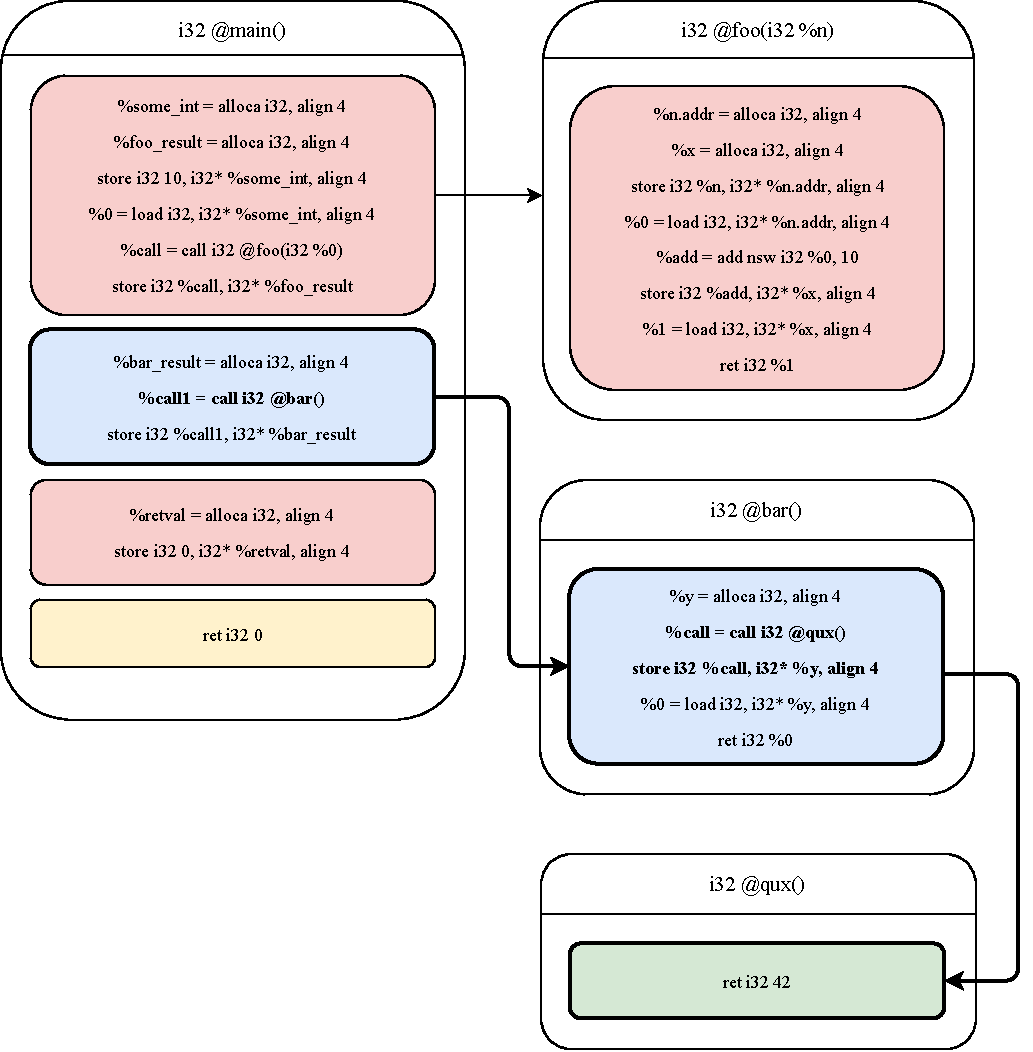
\includegraphics[]{images/example_mod1/example_mod1_removing_prepare.pdf}
    \caption{
    \mintinline{text}{example_mod1.s}:
    Components selected for removal are marked \emph{red}.
    \emph{Yellow} component is not marked for removal, because it contains
    terminator. \emph{Green} component was discovered by the modified algorithm
    and has been added to the path and therefore will not be removed.
    }
    \label{fig:mod1_prepare}
\end{figure}

\clearpage

% mod1 extracted
\begin{figure}[ht]
    \centering
    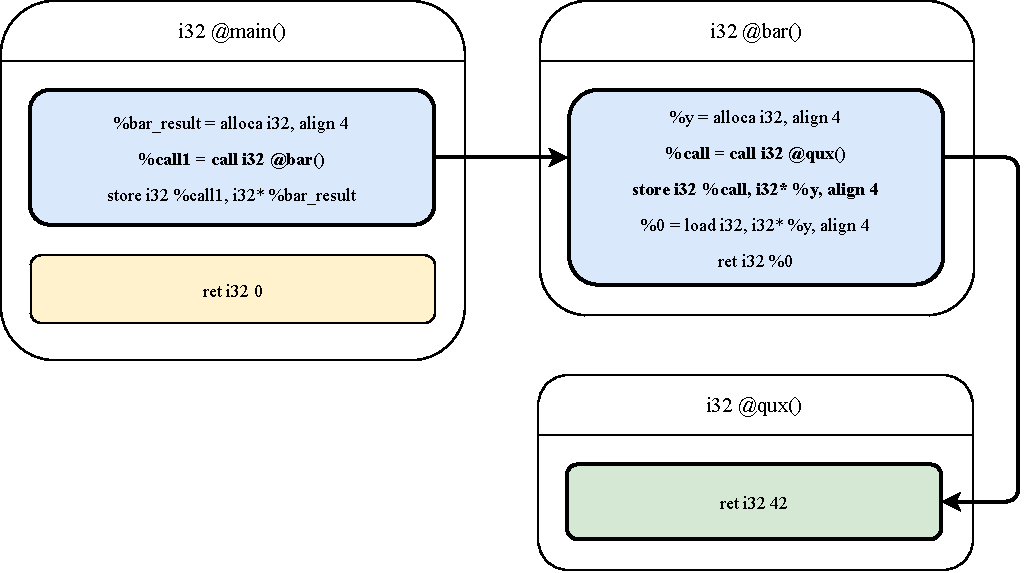
\includegraphics[]{images/example_mod1/example_mod1_removing_done.pdf}
    \caption{
    \mintinline{text}{example_mod1_extracted.s}:
    Final state after removing dead components and functions from
    \mintinline{text}{example_mod1.s}.
    }
    \label{fig:mod1_done}
\end{figure}


% === SUB-SECTION: Branching Instruction =======================================
\subsection{Path Depending on a Branching Instruction}
\label{subsec:path_branching}

Another problem comes with usage of branching instructions.

We now introduce branching into the main function of our exampleas shown in
\mintinline{text}{example_mod2.c}.
The corresponding LLVM IR is shown in the
\mintinline{text}{example_mod2.s}, the branch instruction
occurs at line 42.
Also, there appear two new basic blocks that this branch instruction
refers to:
\mintinline{text}{if.then} and \mintinline{text}{if.end} (lines 44 and 49,
respectively).

If we take a closer look at the generated call graph for
\mintinline{text}{example_mod2.s}
(\autoref{fig:mod2_prepare}), we can observe that the branching instruction
\mintinline{llvm}{br i1 %cmp, label %if.then, label %if.end} is in the
component that is not part of the path. This is problematic, because if we
look at the
\mintinline{text}{example_mod2.c}.
we can clearly see, that in order to get to the target (line 11),
branching needs to be executed and thus included in the path.
We present the algorithm from the previous subsection
(\autoref{subsec:path_function}) with the extension that handles the above
described scenario:

\begin{minted}[label=eliminating dead components - mod2,breaklines,escapeinside=||,frame=lines,framesep=10pt]{text}
0. Let CS = set of all components in the code
1. Let PATH = set of components on the path from source to target
2. FOR EACH component C in PATH:
      FOR EACH instruction I in C:
          IF instruction I is part of basic block handled by the branch instruction:
             FIND component with the branching instruction responsible for I and add it to the PATH
3. Recursively find all called functions that originate from PATH
   using Breath-first search and add them to the PATH.
4. FOR EACH component C in set CS:
      IF component C is not in the set PATH:
         IF component C does not contain terminator:
             Mark component C as DEAD
5. Remove all components marked as DEAD
\end{minted}

As we can see in the
\mintinline{text}{example_mod2.s}, if we examine instruction from the line 45,
we can see that it belongs to the basic block
\mintinline{text}{if.then}.

The call graph for the new program is shown in the \autoref{fig:mod2_prepare}.
We can observe that the instruction from line 45 lies on the path and at the
same time belongs to the basic block \mintinline{text}{if.then}.
This basic block is handled by the branch instruction from line 42.
The modified algorithm
finds a component that contains this branch instruction and adds it to the path.
The call graph with the computed components and the path that the algorithm
takes as the input is shown in \autoref{fig:mod2_prepare}.
The component in the main function marked as green contains a branching
instruction that the algorithm identified as necessary and therefore is was
added to the path.

The result of the algorithm is presented in
\mintinline{text}{example_mod2_extracted.s} and visually in the form of a call
graph \autoref{fig:mod2_done}.


% mod2 C code
\begin{minted}[label=example\_mod2.c,frame=lines,framesep=10pt,linenos]{C}
int foo(int n) {
    int x = n + 10;
    return x;
}

int qux(void) {
    return 42;
}

int bar(void) {
    int y = qux();
    return y;
}

int main(void) {
    int some_int = 10;
    int foo_result = foo(some_int);
    int n = 10;
    if (n < 42) {
        int bar_result = bar();
    }
    return 0;
}
\end{minted}

% mod2 IR

\begin{minted}[label=example\_mod2.s,frame=lines,framesep=10pt,linenos]{llvm}
define i32 @foo(i32 %n) #0 {
entry:
  %n.addr = alloca i32, align 4
  %x = alloca i32, align 4
  store i32 %n, i32* %n.addr, align 4
  %0 = load i32, i32* %n.addr, align 4
  %add = add nsw i32 %0, 10
  store i32 %add, i32* %x, align 4
  %1 = load i32, i32* %x, align 4
  ret i32 %1
}

define i32 @qux() #0 {
entry:
  ret i32 42
}

define i32 @bar() #0 {
entry:
  %y = alloca i32, align 4
  %call = call i32 @qux()
  store i32 %call, i32* %y, align 4
  %0 = load i32, i32* %y, align 4
  ret i32 %0
}

define i32 @main() #0 {
entry:
  %retval = alloca i32, align 4
  %some_int = alloca i32, align 4
  %foo_result = alloca i32, align 4
  %n = alloca i32, align 4
  %bar_result = alloca i32, align 4
  store i32 0, i32* %retval, align 4
  store i32 10, i32* %some_int, align 4
  %0 = load i32, i32* %some_int, align 4
  %call = call i32 @foo(i32 %0)
  store i32 %call, i32* %foo_result, align 4
  store i32 10, i32* %n, align 4
  %1 = load i32, i32* %n, align 4
  %cmp = icmp slt i32 %1, 42
  br i1 %cmp, label %if.then, label %if.end

if.then:                                          ; preds = %entry
  %call1 = call i32 @bar()
  store i32 %call1, i32* %bar_result, align 4
  br label %if.end

if.end:                                           ; preds = %if.then, %entry
  ret i32 0
}
\end{minted}



% mod2 extracted

\begin{minted}[label=example\_mod2\_extracted.s,frame=lines,framesep=10pt,linenos]{llvm}
define i32 @qux() #0 {
entry:
  ret i32 42
}

define i32 @bar() #0 {
entry:
  %y = alloca i32, align 4
  %call = call i32 @qux()
  store i32 %call, i32* %y, align 4
  %0 = load i32, i32* %y, align 4
  ret i32 %0
}

define i32 @main() #0 {
entry:
  %n = alloca i32, align 4
  %bar_result = alloca i32, align 4
  store i32 10, i32* %n, align 4
  %0 = load i32, i32* %n, align 4
  %cmp = icmp slt i32 %0, 42
  br i1 %cmp, label %if.then, label %if.end

if.then:                                          ; preds = %entry
  %call1 = call i32 @bar()
  store i32 %call1, i32* %bar_result, align 4
  br label %if.end

if.end:                                           ; preds = %if.then, %entry
  ret i32 0
}
\end{minted}

% mod2 extracted graph
\begin{figure}[ht]
    \centering
    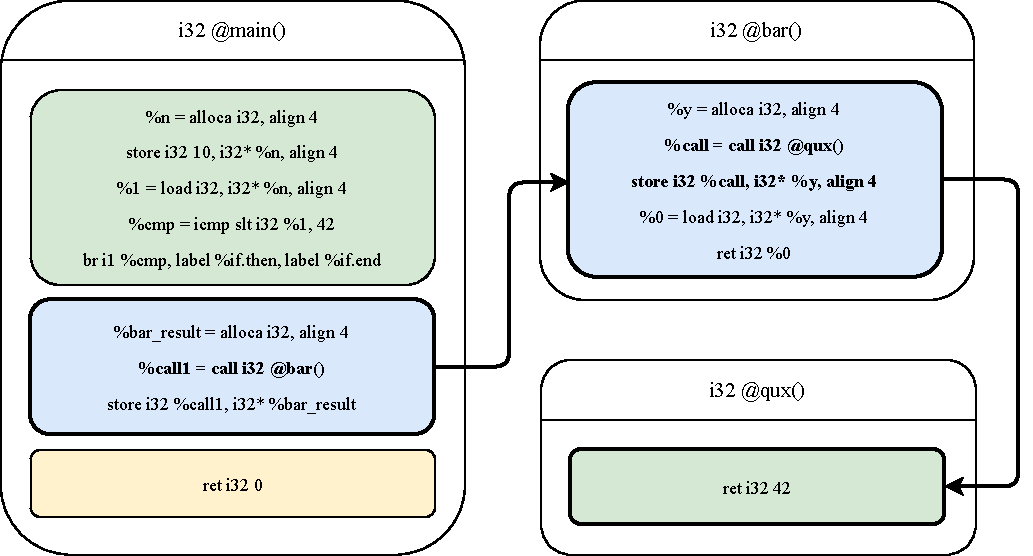
\includegraphics[]{images/example_mod2/example_mod2_removing_done.pdf}
    \caption{
    \mintinline{text}{example_mod2_extracted.s}:
    Final state after removing dead components and functions from
    \mintinline{text}{example_mod2.s}.
    }
    \label{fig:mod2_done}
\end{figure}

% mod2 callgraph
\begin{figure}[ht]
    \centering
    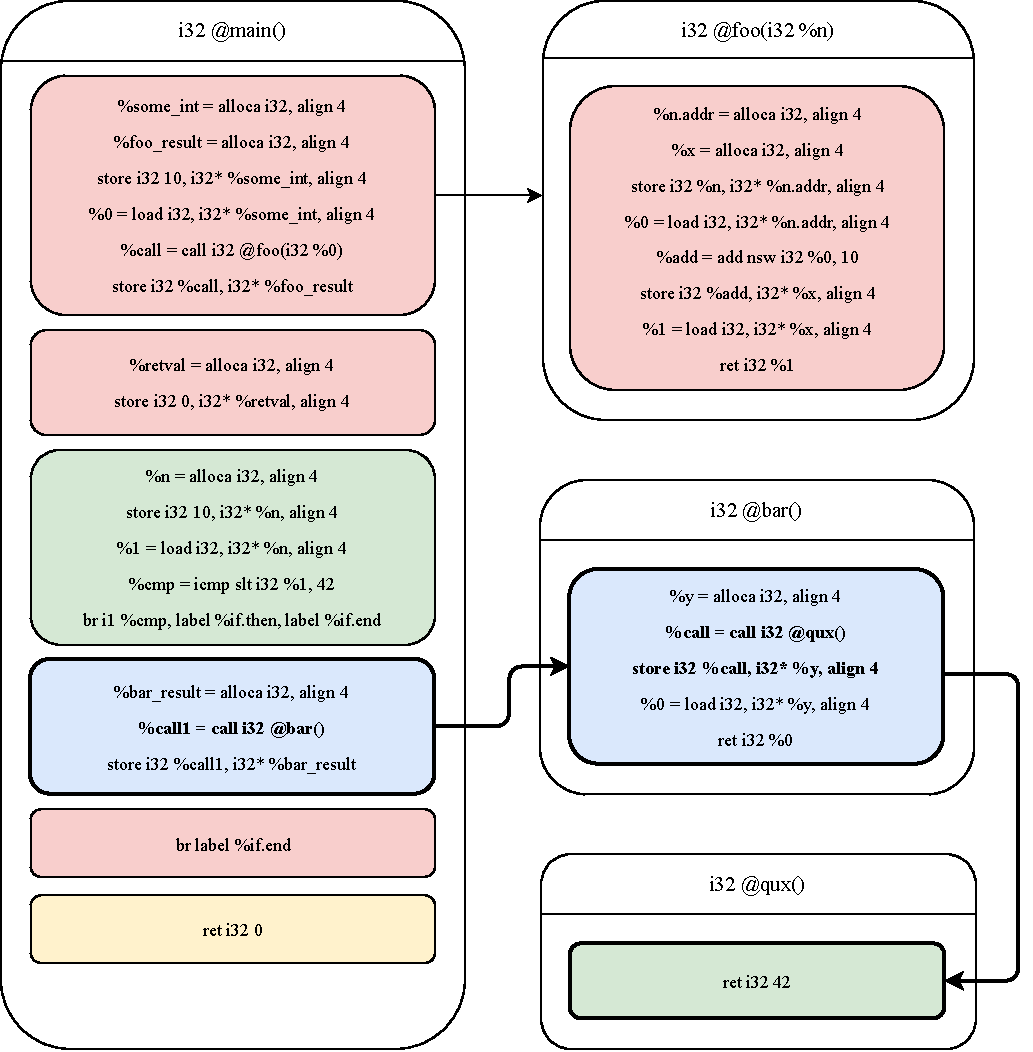
\includegraphics[]{images/example_mod2/example_mod2_removing_prepare.pdf}
    \caption{
    \mintinline{text}{example_mod2.s}:
    Components selected for removal are marked \emph{red}.
    \emph{Yellow} component is not marked for removal, because it a contains
    terminator instruction.
    \emph{Green} components were discovered by the modified
    algorithm and were added to the path and therefore will not be removed.
    }
    \label{fig:mod2_prepare}
\end{figure}



% === CHAPTER: Implementation ==================================================
\chapter{Implementation}
\label{chap:implementation}

% === SECTION: APEXPass ========================================================
\section{APEXPass}
\label{sec:impl_apexpass}

% intro
The method that we described in the \autoref{chap:design} is implemented as a
LLVM pass called \textbf{APEXPass}.
We have decided to implement the method as an pass because of the great
capabilities of the LLVM infrastructure. Leveraging LLVM, APEXPass can be ran
as an optimization step along with other LLVM optimizations or executed
separately with LLMV optimizer tool opt:

\begin{minted}[frame=lines,framesep=10pt,breaklines]{bash}
opt -o apex.bc -load libAPEXPass.so -apex -file=example.c -line=7 < example.bc 2> build/apex.log
\end{minted}

% apexpass input & output definition
Using opt command presented above, APEXPass is ran via \textbf{apex} flag and defines
two command line arguments: file and line.
Argument \textbf{file} specifies the C source file where is the target located
(in our case example.c) and argument \textbf{line} specifies number of the line
in the file (in the example, line number 7).

Input to the opt is the example.bc, which is the bitcode representation of the
example.c with included source-level debug information. The reason why we need
debug information included in the example.bc is explained in the
\autoref{sec:impl_inst_locate}.

We can get example.bc by compiling example.c using clang:

\begin{minted}[frame=lines,framesep=10pt]{bash}
clang -g -c -emit-llvm example.c -o example.bc
\end{minted}

Another necessary input to the opt is \textbf{libAPEXPass.so}. It is the pass
itself compiled into the shared library.

APEXPass produces output \textbf{apex.bc}, which is the bitcode representation
of the extracted part from the example.bc.
This extracted program can be executed directly with the tool lli as follows:

\begin{minted}[frame=lines,framesep=10pt]{bash}
lli apex.bc
\end{minted}

APEXPass can be defined within the LLVM framework as a \textbf{ModulePass}
because it derives from the ModulePass class.\footnote{
\url{https://llvm.org/doxygen/classllvm_1_1ModulePass.html}
}

There are other pass clases besides ModulePass (FunctionPass, LoopPass,
RegionPass, BasicBlockPass, etc.), but we have decided to implement APEXPass as
a ModulePass because it is the most general class of passes and thus provides
the greatest flexibility.

There are some disadvantages that comes to implementing pass as an ModulePass.
To name a few, function bodies are are referred by no particular order.
Also, there are no possible
optimizations to be done for ModulePass because optimizer does not have enough
information about its behaviors. \cite{llvm-module-pass}

However, these disadvantages are not critical for our purposes and advantages
of having whole program abstracted as a single unit outweigh the disadvantages.

% === SUB-SECTION: APEXPass structure ==========================================
\subsection{Structure of the APEXPass}

In order to work correctly, each ModulePass has to override runOnModule method
with the following signature:

\mintinline{C}{
virtual bool runOnModule(Module &M) = 0;
}

This method is the main part of the pass and performs computation of the pass.
All five steps that we described in the \autoref{sec:method_overview} are going
to be part of the \mintinline{C}{runOnModule} method.
In this section, we are going to explain
additional, implementation specific steps that needed to be added to
the method.

We add three additional steps on top of the original five method steps
described in the \autoref{sec:method_overview} (step 1, 7 and 8). We also
explain implementation specific details behind step 2 in the subsequent
subsection.

The APEXPass structure therefore looks like this:

% apexpass structure
\begin{myItemize}
\item{\mintinline{C}{runOnModule()}:}

\begin{myEnumerate}
\item{\textbf{Locate target instructions that map to the user input.}}
\item \textbf{Run dg.} Compute data dependencies between instructions.
\item Find connected components in the computed data dependencies inside
every function.
\item Construct call graph, mapping between connected components and functions
that are being called from these components.
\item Find path from source to target in the call graph.
\item Eliminate dead components and functions that do not depend on the path.
\item{\textbf{Inject exit and extract function calls into the code.}}
\item{\textbf{Strip debug symbols from the extracted code.}}
\end{myEnumerate}

\end{myItemize}


% === SUB-SECTION: Locating Target Instructions ================================
\subsection{Locating Target Instructions}
\label{sec:impl_inst_locate}

Since APEXPass, or generally any LLVM pass, does not work directly with the C
code but instead works with the LLVM IR, we need a procedure for mapping
C source code to the IR.

As we mentioned in the \autoref{sec:method_example}, we know precise position
of the target in the example.c, but we do knot know exectly what IR
instructions are equivalent to the target.

Taking example from the \autoref{sec:method_example}, we have input program
example.c and target in the function bar at the line 7.

The target in the example.c is the following line of code:
\mintinline{C}{int y = 42;}
which is represented by the following IR instruction in the example.s:

\mintinline{llvm}{
store i32 42, i32* %y, align 4
}

The way we achieve mapping between original C source code and IR is by
using source-level debug information that is introduced by the compiler
(usually with the -g flag).
The example.s with debug symbols is shown in the \autoref{appendix:example_dbg}.
Once the example.s is compiled with debug information, we can iterate from within
the APEXPass over each instruction to find out its parent file name and
line number using the following code:\cite{llvm-dbg}

\begin{minted}[frame=lines,framesep=10pt]{cpp}
for (const auto &function : module) {
    for (const auto &basic_block : function) {
        for (const auto &instruction : basic_block) {
            if (DILocation *Loc = instruction->getDebugLoc()) {
                unsigned Line = Loc->getLine();
                StringRef File = Loc->getFilename();
            }
        }
    }
}
\end{minted}

Once the Line and File match with the user input, we have found our target
IR instruction.

Depending on how complex the target line of code is, there may be more than one
IR instructions associated with it. For example, taking the target line number
7 from the example.c:

\mintinline{C}{
int y = 42;
}

IR instruction that maps to it is the following:

\mintinline{llvm}{
store i32 42, i32* %y, align 4
}

However, when we take as a target line number 2 from the example.c:

\mintinline{C}{
int x = n + 10;
}

Then, the mapping will be to the three following IR instructions:

\begin{minted}[frame=lines,framesep=10pt]{llvm}
%0 = load i32, i32* %n.addr, align 4
%add = add nsw i32 %0, 10
store i32 %add, i32* %x, align 4
\end{minted}

\mintinline{C}{int x = n + 10;} is much more complex line of code than
\mintinline{C}{int y = 42;} and thus, is represented by more IR instructions.


% === SUB-SECTION: Computing Data Dependencies With dg =========================
\subsection{dg - Computing Data Dependencies}

As we have mentioned in the \autoref{sec:design-dep}, we have not implemented
data dependency computation in the APEXPass itself.
Instead, we use open-source tool by Marek Chalupa called \textbf{dg}\footnote{
\url{https://github.com/mchalupa/dg}
}
to compute data dependencies and get the results that we described in the
\autoref{sec:design-dep}.

\emph{Dg is a library which implements dependence graphs for programs. It
contains a set of generic templates that can be specialized to user's needs.
As a part of dg, you can find pointer analyses, reaching definitions analysis
and a static slicer for LLVM.}\cite{dg-github}

Since dg is extensive project that covers more than we need, we use just
some parts of it, especially LLVMDependenceGraph. This structure provides
data dependencies which APEXPass requires.

% === SUB-SECTION: Injecting Exit and Extract Functions to the Code ============
\subsection{Injecting Exit and Extract Functions}
\label{sub:impl_inject}

After having found the target instruction, we need to ensure that the execution
of the extracted program stops right after the target has been reached.
We do not want to execute program after it reached the target, because it is
contradictory to what our method should do.
We also want to extract value of the target and provide this information to the
user.

In order to accomplish this, we need to inject the following three additional
instructions right after the target:

\begin{myItemize}
\item Load instruction X that takes value of the target and stores it into
the separate register.
\item Call instruction to extract function with X as an function argument.
\item Call instruction to exit function which will terminate execution.
\end{myItemize}

Taking example\_extracted.s from the \autoref{sec:method_example} (with target
\mintinline{llvm}{store i32 42, i32* %y, align 4}) and injecting exit and
extract functions after the target gives the final result presented in the
example\_extracted\_final.s code:

\begin{minted}[label=example\_extracted\_final.s,frame=lines,framesep=10pt,linenos]{llvm}
define i32 @bar() #0 {
entry:
  %y = alloca i32, align 4
  store i32 42, i32* %y, align 4
  %_apex_extract_int_arg = load i32, i32* %y
  call void @_apex_extract_int(i32 %_apex_extract_int_arg)
  call void @_apex_exit(i32 0)
  %0 = load i32, i32* %y, align 4
  ret i32 %0
}

define i32 @main() #0 {
entry:
  %bar_result = alloca i32, align 4
  %call1 = call i32 @bar()
  store i32 %call1, i32* %bar_result, align 4
  ret i32 0
}
\end{minted}

As we can see on the lines 5,6 and 7, there are three new instructions injected
right after the target. Instructions at lines 6 and 7 are call instructions
to the extract and exit functions.
Because these instructions call external functions, their definitions has to be
linked to the program. This is done by the apex.py and is discussed in the
\autoref{sec:impl_launcher}.

Exit function \mintinline{text}{_apex_exit} and extract function
\mintinline{text}{_apex_extract_int} are implemented in the library
\mintinline{text}{apexlib.c}:

\begin{minted}[label=apexlib.c,frame=lines,framesep=10pt,linenos]{C}
#include <stdio.h>
#include <stdlib.h>

void _apex_exit(int exit_code) {
  exit(exit_code);
}

void _apex_extract_int(int i) {
  printf("%d", i);
}
\end{minted}

Extraction is limited by the type of extracted value. By looking at the
\mintinline{text}{example extracted final.s}, we can observe that the
type of \mintinline{llvm}{%y} is \mintinline{llvm}{i32} (integer).
We have to call extraction function that accepts argument of this type.
Current implementation supports only extraction of values with the integer type
(more specifically \mintinline{llvm}{i32}).


% === SUB-SECTION: Stripping Debug Symbols =====================================
\subsection{Stripping Debug Symbols}

The last step that APEXPass performs is stripping debug information from the
final code.
The reason why we do this step is to be sure that the final extracted program
is in the consistent state. APEXPass works with the code that contains debug symbols.
Problem is that the three new injected instructions that were presented in the
\autoref{sub:impl_inject} are without debug symbols. Having parts of the code
with debug symbols and other parts without creates inconsistent state.
Program in this inconsistent state would not be possible to compile into
bitcode without issues.

There are two approaches that could resolve this issue:
\begin{myEnumerate}
\item{Add debug information to each new instruction that we insert into the code.}
\item{Strip all debug information from the code.}
\end{myEnumerate}

We have picked the second option, because it is sufficient to ensure code
consistency and because of the ease of the implementation. LLVM provides API\footnote{
\url{https://llvm.org/doxygen/DebugInfo_8cpp_source.html\#l00314}
}
for stripping debug information from function, therefore we can use the following
code to strip all debug information from the entire program:

\begin{minted}[frame=lines,framesep=10pt]{cpp}
for (auto &Function : Module) {
    llvm::stripDebugInfo(Function);
}
\end{minted}

% === SECTION: Launcher ========================================================
\section{APEX}
\label{sec:impl_launcher}

We have integrated APEXPass into the open-source tool called APEX, which is
freely accessible in the repository: \url{https://github.com/examon/APEX}.
APEX serves as an user-friendly wrapper around APEXPass
while providing an easy way to run APEXPass without leaving user to
worry about the internal structure.

% === SUB-SECTION: apex.py =====================================================
\subsection{apex.py}

There are multiple steps that need to be executed in order to properly
run APEXPass. Therefore, we have implemented script apex.py that simplifies
this process to the absolute minimum.

Running APEXPass via launcher apex.py does require only python3. The following
example demonstrates how to run APEXPass with the input example.bc, with target
located in the file example.c on the line 2.

\begin{minted}[frame=lines,framesep=10pt]{bash}
python apex.py example.bc example.c 2 --export=true
\end{minted}

apex.py launcher has three mandatory command line arguments and one optional.
First argument is input code in the llvm bitcode format. Second argument is the
target file and third is target line of code in the file.
Optional argument is boolean flag and when set to true, apex.py will
export call graphs of the input and also the extracted program.

Upon finishing execution, apex.py will create executable called
\textbf{extracted}. This executable contains extracted part of the program and
can be run just like any unix executable:

\mintinline{text}{
./extracted
}

Besides producing exected executable, apex.py creates build directory with the
following important files:

\begin{myItemize}
\item apex.bc: Extracted program in the llvm bitcode format that can be run separately
via tool lli.
\item apex.out: Output of the apex.bc.
\item apex.log: Log produced by the APEXPass.
\end{myItemize}

% === SUB-SECTION: linking apexlib =============================================
\subsection{Linking apexlib and Input}

The important step in the apex.py execution is linking apexlib with the user
input. Linking has to be done because apexlib defines exit and extract
functions and these functions need to be injected after the target
(\autoref{sub:impl_inject}).

Linking itself is performed in the following three setps:
\begin{myEnumerate}
\item Compile apexlib.c into the LLVM bitcode apexlib.bc.

\mintinline{text}{clang -g -c -emit-llvm apexlib.c -o apexlib.bc}

\item Link apexlib.bc with the user input (e.g. example.bc) and produce linked.ll
IR code.

\mintinline{text}{llvm-link apexlib.bc example.bc -S -o=linked.ll}

\item Run assember on the linked.ll and produce bitcode linked.bc.

\mintinline{text}{llvm-as build/linked.ll -o build/linked.bc}

\end{myEnumerate}

These three steps will essentially take user input example.bc, link to it
library with the exit and extract functions apexlib.bc and produce output
linked.bc that will now serve as an input to the APEXPass instead of the original
input example.bc.

linked.ll is available for comparison with example.s in the
\autoref{appendix:linked}.

% === CHAPTER: Experiments =====================================================
\chapter{Experiments}
\label{chap:experiments}

We present four experiments in this chapter. The aim of the experiments is to
test APEX on various inputs and determine if the implementation can handle
extracting parts from the basic programs. We perform extractions on various
targets and evaluate the results.

To demonstrate APEX capabilities, we perform tests on one artificially created
program and three well know UNIX utilities.

% === SECTION: example_mod2.c ==================================================
\section{\mintinline{text}{example_mod2.c}}
\label{sec:exp_test}

The first experiment is conducted on the code example\_mod2.c, which we
introduced in \autoref{subsec:path_branching}. We picked this simple code
in order to demonstrate the whole process of testing APEX capabilities.

\begin{minted}[label=example\_mod2.c,frame=lines,framesep=10pt,linenos]{C}
int foo(int n) {
    int x = n + 10;
    return x;
}

int qux(void) {
    return 42;
}

int bar(void) {
    int y = qux();
    return y;
}

int main(void) {
    int some_int = 10;
    int foo_result = foo(some_int);
    int n = 10;
    if (n < 42) {
        int bar_result = bar();
    }
    return 0;
}
\end{minted}

First, we compile example\_mod2.bc into the LLVM bitcode with debug
information:

\mintinline{shell}{
clang -c -g -emit-llvm example_mod2.c -o example_mod2.bc
}

We run -dot-callgraph pass via opt tool and dot with the following commands to
generate call graph image from the example\_mod2.bc
(\autoref{fig:exp_img_mod2}):

\mintinline{shell}{
opt -dot-callgraph example_mod2.bc && dot callgraph.dot -Tsvg -O
}

% call graph before linking
\begin{figure}[ht]
    \centering
    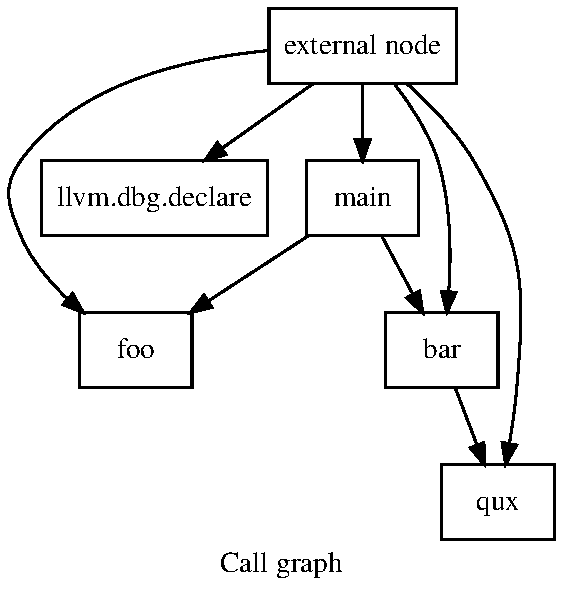
\includegraphics[width=0.5\textwidth]{images/experiments/mod2.pdf}
    \caption{
    \mintinline{text}{example_mod2.c}
    call graph before linking and running APEXPass.
    }
    \label{fig:exp_img_mod2}
\end{figure}

\autoref{fig:exp_img_mod2} serves as as reference for the subsequent stages of
this experiment.
Having compiled input with debug symbols successfully, we fulfilled
requirements for APEX input and can therefore run apex.py to start extraction.

% target 16
\begin{minted}[label=extraction with target line number 16, frame=lines,framesep=10pt,breaklines]{shell}
> python apex.py example_mod2.bc example_mod2.c 16
> ./extracted
10
\end{minted}

APEX generated binary \mintinline{text}{extracted} with respect to the target
at the line number 16. When executing extracted binary, we get value of the
\mintinline{text}{some_int} via injected function
\mintinline{text}{_apex_extract_int} (which is 10).
Execution subsequently stops because
\mintinline{text}{_apex_exit} is called. APEX also generated build/apex.bc
file, which is the extracted program in the LLVM bitcode format. We can generate
the call graph using the same method as we did with the example\_mod2.bc and
get \autoref{fig:exp_img_mod2_target16}.

% call graph after apex, target 16
\begin{figure}[ht]
    \centering
    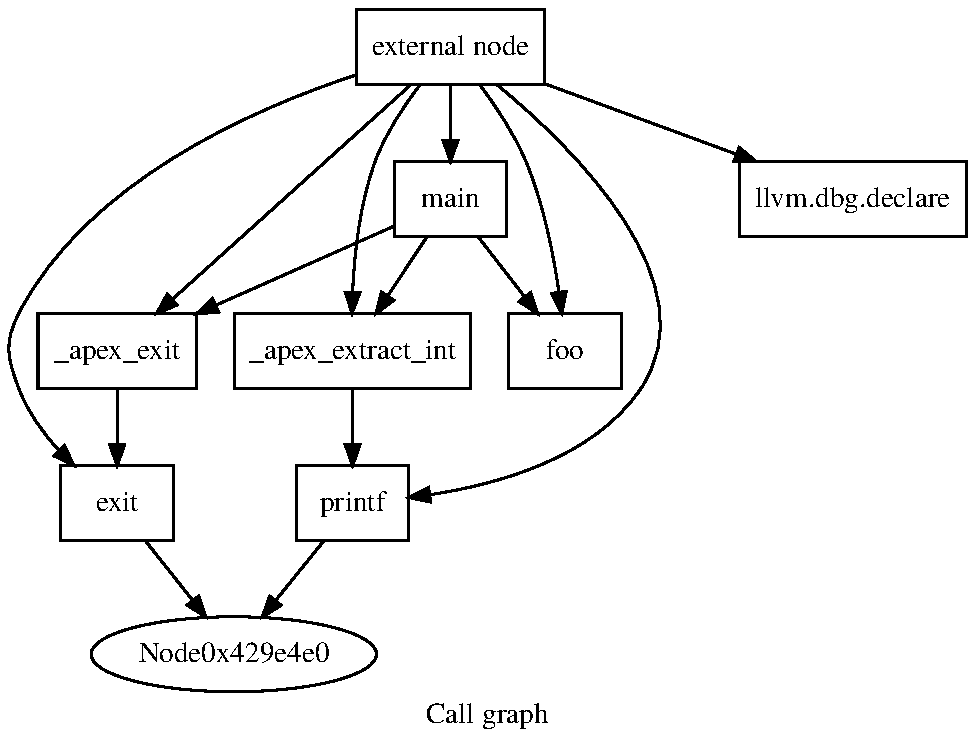
\includegraphics[width=0.75\textwidth]{images/experiments/mod2_target16.pdf}
    \caption{
    \mintinline{text}{example_mod2.c}: call graph after extraction with target
    at the line 16.
    }
    \label{fig:exp_img_mod2_target16}
\end{figure}

We can see, that the generated call graph includes functions
from apexlib, namely \mintinline{text}{_apex_exit} and
\mintinline{text}{_apex_extract_int}.

When comparing \autoref{fig:exp_img_mod2} and
\autoref{fig:exp_img_mod2_target16} we observe, that functions bar and qux are
deleted. APEXPass determined that they do not need to be part of the final
extracted executable and therefore dropped them from the code.



% === SECTION: yes.c ===========================================================
\section{\mintinline{text}{yes.c}}
\label{sec:exp_yes}

The following experiment will be conducted on the classic UNIX utility called
yes.
yes repeatedly outputs a line with specified string or 'y' until
killed.

We use source code from the open-source implementation of yes
from the following repository: \url{https://github.com/mubaris/yes}

Full C source code that implements yes is shown in the yes.c listing:

\begin{minted}[label=yes.c,frame=lines,framesep=10pt,linenos]{C}
#include <stdio.h>
#include <stdlib.h>
#include <string.h>

#define max(a,b) \
    ({ __typeof__ (a) _a = (a); \
     __typeof__ (b) _b = (b); \
     _a > _b ? _a : _b; });

int main(int argc, char* argv[]) {
    char* output;
    int output_size;
    int output_len;

    if (argc > 1) {
        // Create buffer.
        int needed_size = 2 + strlen(argv[1]);
        for (int i = 2; i < argc; i++) {
            needed_size += 1 + strlen(argv[i]);
        }

        output = (char*) malloc(needed_size);

        // Append to buffer.
        strcat(output, argv[1]);
        for (int i = 2; i < argc; i++) {
            strcat(output, " ");
            strcat(output, argv[i]);
        }
        strcat(output, "\n");
        output_len = strlen(output);
    } else {
        output = "y\n";
        output_len = 2;
    }

    // Flood.
    for(;;)
        fwrite(output, 1, output_len, stdout);
}
\end{minted}

After compilation yes.c into the bitcode yes.bc, we pick
\mintinline{C}{int needed_size} from line 17 as a target.

\begin{minted}[label=extraction with target line number 17, frame=lines,framesep=10pt]{shell}
> python apex.py yes.bc yes.c 17
> ./extracted foo
5
> ./extracted foobar
8
> ./extracted
y
y
y
...
\end{minted}

Extracted program correctly outputs the value of the
\mintinline{C}{int needed_size} when we provide some command line argument.
It also correctly executes the branch else when we do not provide any command
line argument.

Next, we pick line 31 as a target, which corresponds to the line
\mintinline{C}{output_len = strlen(output);}.
Running apex.py, we get the following output when executing extracted binary:

\begin{minted}[label=extraction with target line number 31,frame=lines,framesep=10pt]{shell}
> python apex.py yes.bc yes.c 31
> ./extracted foo
4
> ./extracted foobar
7
> ./extracted
y
y
y
...
\end{minted}

Finally, lets test the else branch of the yes.c by picking line 34 as a target:
(\mintinline{C}{output_len = 2;}):

\begin{minted}[label= extraction with target line number 34,frame=lines,framesep=10pt]{shell}
> python apex.py yes.bc yes.c 34
> ./extracted foo
foo
foo
foo
...
> ./extracted
2
\end{minted}

From the performed experimentation, we can conclude that APEX can handle inputs
with the complexity of the yes.c source code.

% === SECTION: domainname.c=====================================================
\section{\mintinline{text}{domainname.c}}
\label{sec:exp_domainname}

Second UNIX utility that we use for testing is domainname, which is used
for showing or setting the system's NIS/YP domain name.

We use the following open-source implementation of domainname provided by the
OpenBSD community:
\url{https://raw.githubusercontent.com/openbsd/src/master/bin/domainname/domainname.c}


\begin{minted}[label=domainname.c,frame=lines,framesep=10pt,linenos]{C}
#include <err.h>
#include <stdio.h>
#include <stdlib.h>
#include <string.h>
#include <unistd.h>
#include <limits.h>

char *__progname;
void usage(void);

int
main(int argc, char *argv[])
{
    int ch;
    char domainname[HOST_NAME_MAX+1];

    while ((ch = getopt(argc, argv, "")) != -1)
        switch (ch) {
        default:
            usage();
        }
    argc -= optind;
    argv += optind;

    if (argc > 1)
        usage();

    if (*argv) {
        if (setdomainname(*argv, strlen(*argv)))
            err(1, "setdomainname");
    } else {
        if (getdomainname(domainname, sizeof(domainname)))
            err(1, "getdomainname");
        (void)printf("%s\n", domainname);
    }
    return(0);
}


void usage(void)
{
    (void)fprintf(stderr, "usage: %s [name-of-domain]\n", __progname);
    exit(1);
}
\end{minted}

Picking target \mintinline{C}{argc -= optind;} from line 22, we get the
following results:

\begin{minted}[label=extraction with target line number 22,frame=lines,framesep=10pt]{shell}
python apex.py domainname.bc domainname.c 22
> ./extracted
0
> ./extracted a b
2
> ./extracted a b c d
4
\end{minted}

Interestingly, since we targeted \mintinline{C}{argc} variable, it looks like
the extracted executable counts number of supplied command line arguments.

% === SECTION: sleep.c =========================================================
\section{\mintinline{text}{sleep.c}}
\label{sec:sleep}

Last UNIX utility that we test is sleep.
This utility produces delay for a specified amount of time.

We use the following open-source implementation of sleep provided by the
OpenBSD community:
\url{https://raw.githubusercontent.com/openbsd/src/master/bin/sleep/sleep.c}

\begin{minted}[label=domainname.c,frame=lines,framesep=10pt,linenos]{C}
#include <ctype.h>
#include <signal.h>
#include <stdio.h>
#include <stdlib.h>
#include <time.h>
#include <unistd.h>
#include <err.h>

extern char *__progname;
void usage(void);
void alarmh(int);

int
main(int argc, char *argv[])
{
    int ch;
    time_t secs = 0, t;
    char *cp;
    int nsecs = 0;
    struct timespec rqtp;
    int i;

    signal(SIGALRM, alarmh);

    while ((ch = getopt(argc, argv, "")) != -1)
        switch(ch) {
        default:
            usage();
    }
    argc -= optind;
    argv += optind;

    if (argc != 1)
        usage();

    cp = *argv;
    while ((*cp != '\0') && (*cp != '.')) {
        if (!isdigit((unsigned char)*cp))
            errx(1, "seconds is invalid: %s", *argv);
        t = (secs * 10) + (*cp++ - '0');
        if (t / 10 != secs)	/* oflow */
            errx(1, "seconds is too large: %s", *argv);
        secs = t;
    }

    /* Handle fractions of a second */
    if (*cp == '.') {
        cp++;
        for (i = 100000000; i > 0; i /= 10) {
            if (*cp == '\0')
                break;
            if (!isdigit((unsigned char)*cp))
                errx(1, "seconds is invalid: %s", *argv);
            nsecs += (*cp++ - '0') * i;
        }

        while (*cp != '\0') {
            if (!isdigit((unsigned char)*cp++))
                errx(1, "seconds is invalid: %s", *argv);
        }
    }

    while (secs > 0 || nsecs > 0) {
        if (secs > 100000000) {
            rqtp.tv_sec = 100000000;
            rqtp.tv_nsec = 0;
        } else {
            rqtp.tv_sec = secs;
            rqtp.tv_nsec = nsecs;
        }
        if (nanosleep(&rqtp, NULL))
            err(1, NULL);
        secs -= rqtp.tv_sec;
        nsecs -= rqtp.tv_nsec;
    }
    return (0);
}

void
usage(void)
{
    (void)fprintf(stderr, "usage: %s seconds\n", __progname);
    exit(1);
}

void
alarmh(int signo)
{
    _exit(0);
}
\end{minted}

By picking target \mintinline{text}{nsecs += (*cp++ - ’0’) * i;} at line 54, we
get the following results:

\begin{minted}[label=extraction with target line number 54,frame=lines,framesep=10pt]{shell}
python apex.py sleep.bc sleep.c 54
> ./extracted foo
extracted: seconds is invalid: foo
> ./extracted 3
...
(sleeps 3 seconds)
...
> ./extracted 3.14
100000000
> ./extracted
Segmentation fault (core dumped)
\end{minted}

Running extracted with string or integer argument produces the expected
behavior (error and sleeping).
When running extracted executable with command line argument encompassing
decimal point, the execution hits our target at the line 54. Value of the
\mintinline{C}{nsecs} is extracted via \mintinline{text}{_apex_extract_int}
function and printed as expected.

The interesting thing happens when we run extracted binary without any
command line arguments.
If we look into sleep.c, we can see that in the case where there are no command
line arguments, usage function should be called.
However, because we have picked target at the line 54, APEXPass determined that
it is safe to remove function usage from the code (which is the case when we
run binary with command line arguments).

If we compare call graphs \autoref{fig:exp_img_sleep} and
\autoref{fig:exp_img_sleep_target54}, we can see that the function usage has
been removed and is no longer part of the extracted binary.

\begin{figure}[ht]
    \centering
    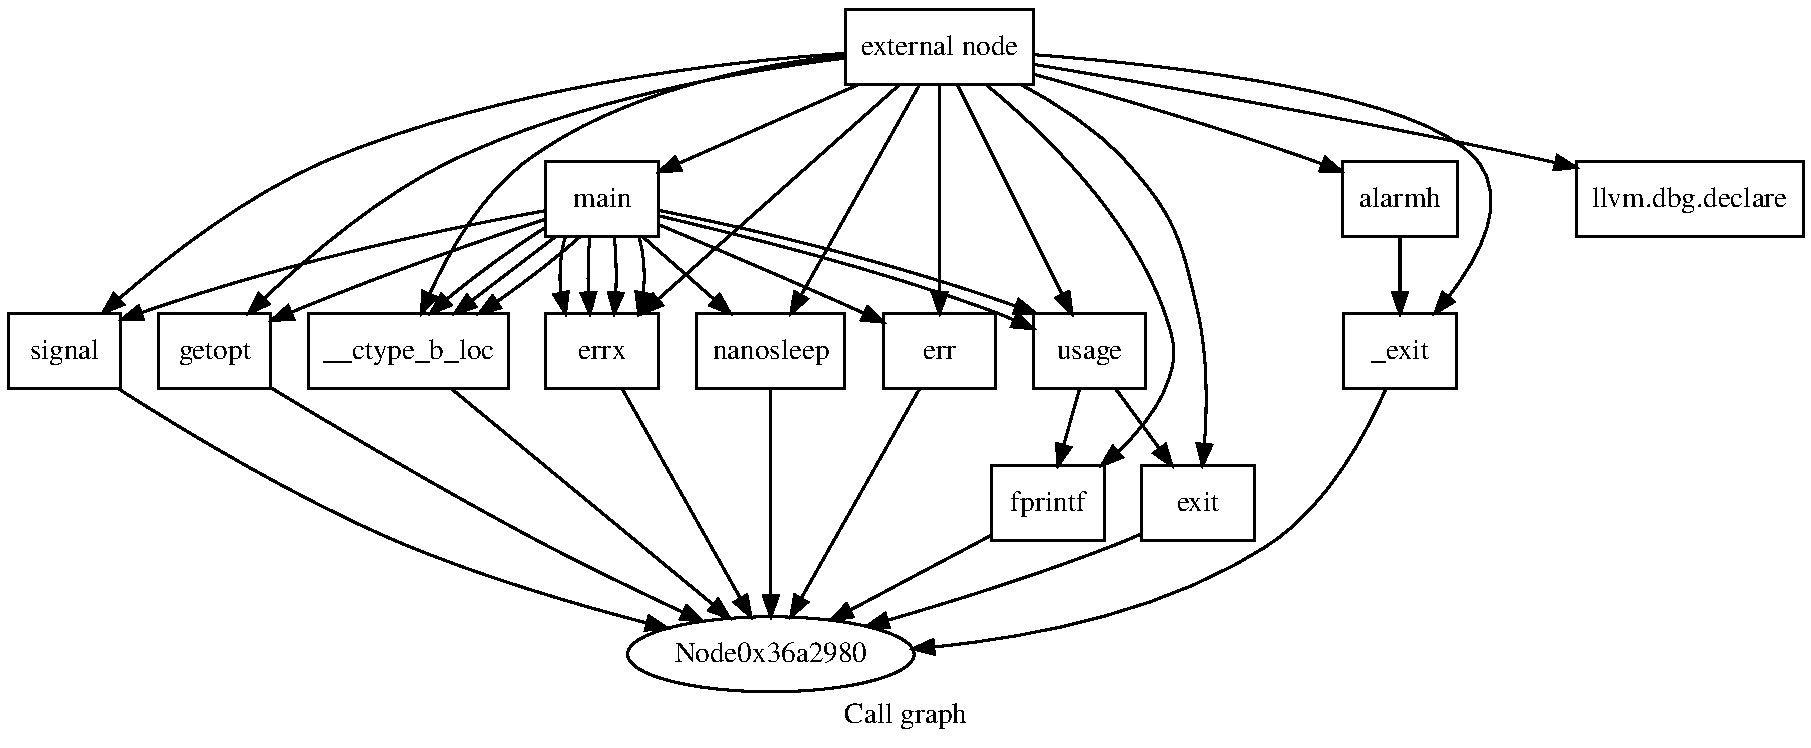
\includegraphics[width=1\textwidth]{images/experiments/sleep.pdf}
    \caption{
    \mintinline{text}{sleep.c}
    call graph before linking and running APEXPass.
    }
    \label{fig:exp_img_sleep}
\end{figure}

\begin{figure}[ht]
    \centering
    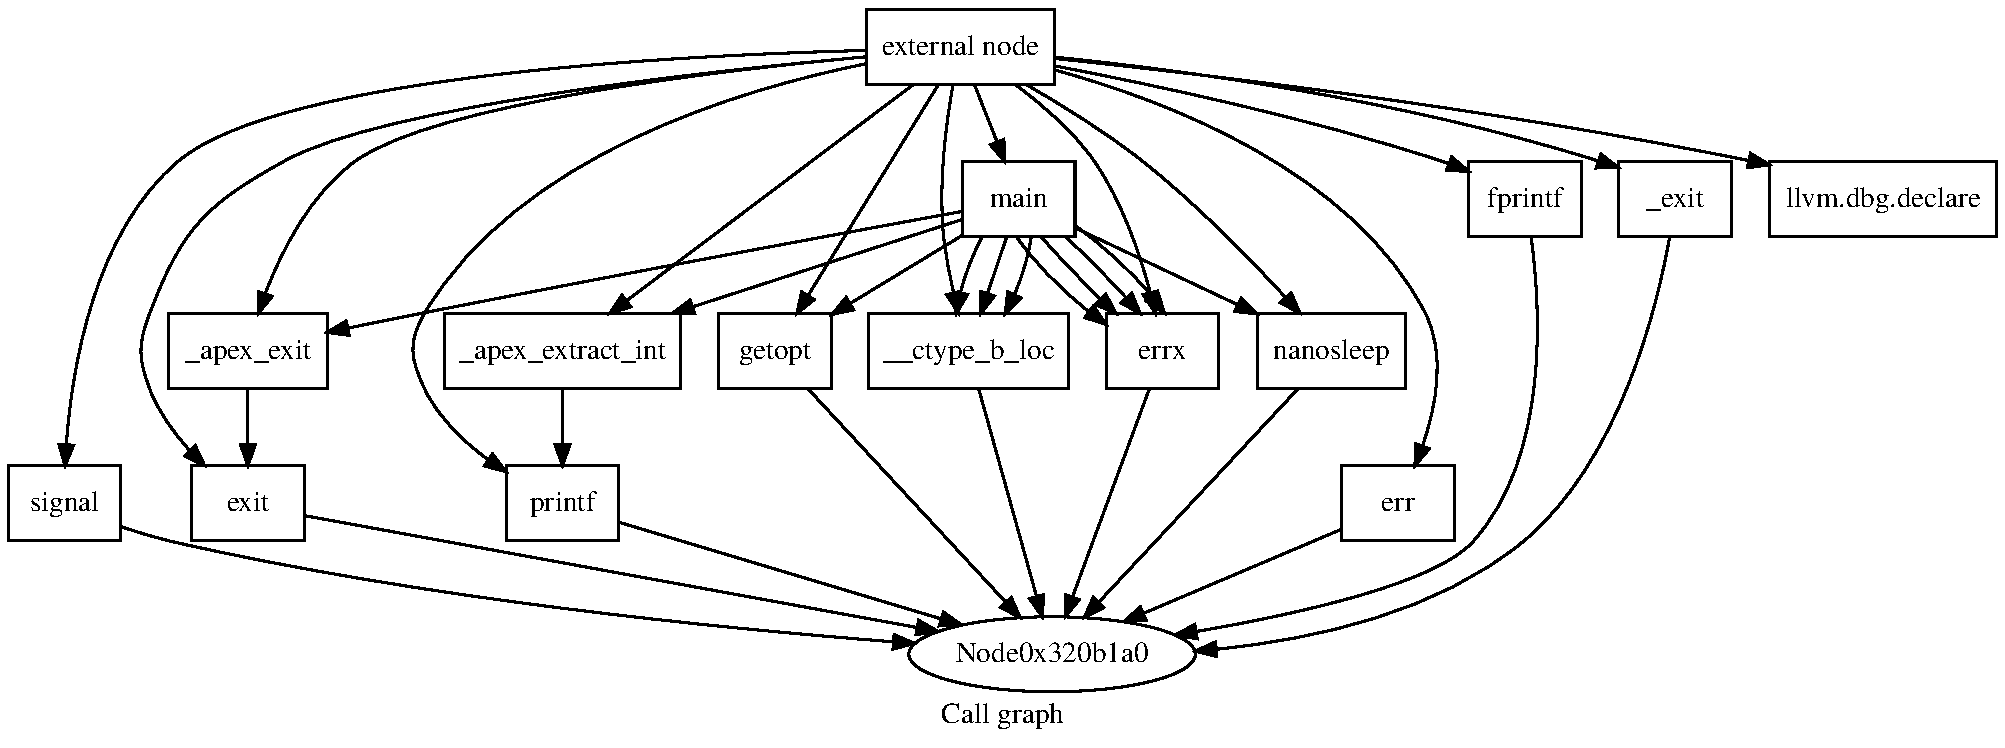
\includegraphics[width=1\textwidth]{images/experiments/sleep_target54.pdf}
    \caption{
    \mintinline{text}{sleep.c}
    call graph after extraction with target at the line 54.
    }
    \label{fig:exp_img_sleep_target54}
\end{figure}



% === CHAPTER: Conclusions =====================================================
\chapter{Conclusions}
\label{chap:conclusions}

In this thesis, we presented the method of extacting parts of programs into
separate binaries. We explained steps and algorithms that the method
performs to achieve the desired extraction.

We developed a LLVM transform pass (APEXPass) implementing the presented
method by leveraging the LLVM infrastructure.
APEXPass was integrated into the open-source tool APEX, which provides the
user-fiendly experience.

Lastly, we have tested APEX on one artifically created program and three
classic UNIX tools. Experiments showed, that the method implemented in the APEX
is sufficient for extracting parts of programs from simple inputs that are
comparable in complexity to small UNIX tools.


% focus on our specific contributions
% focus on the wider view, what this thesis brought to the world

% === SECTION ===
\section{Further Research and Development}
\label{sec:conclusions-next}


As we mentioned in the \autoref{sub:impl_inject}, extraction is currently
limited by the type of the extracted value.
Possible improvement of the extraction procedure would be to implement
extraction functions for every IR type and thus extending apexlib.c.
Implementing algorithm able to determine what type of extraction
function is needed would be crucial in order to support all value types
for extraction.

Path finding procedure that we described in \autoref{sec:design-path} could be
improved by finding multiple paths (not only one) and picking the best fitting
one for the extraction. The best fitting path could be determined by some
optimization criteria (e.g. shortest path, path without fewest external
dependencies, etc.).

Another very useful improvement would be to extend coverage of the dead
code elimination procedure explained in \autoref{sec:design-removing}.
We have already presented two extensions to this procedure
(\autoref{subsec:path_function} and \autoref{subsec:path_branching}).
Designing even more extensions would allow the method to cover more
complex IR code than now and thus would allow extraction from more complicated
C programs.


% === BIBLIOGRAPHY =============================================================
\appendix

% print complete bibliography
\printbibliography

% === CHAPTER ==================================================================
\chapter{Archive structure}
\label{appendix:archive}

Archive contains APEX source code. Upstream version of the APEX can be found in
the repository: \url{https://github.com/examon/APEX}

Please refer to the \mintinline{text}{README.md} for instructions about building
and running APEX.

Example source codes used in this thesis are included in the directory
\mintinline{text}{examples}.


% === APPENDIX: example.s ======================================================
\chapter{example.s}
\label{appendix:example}

\begin{minted}[frame=lines, framesep=10pt, breaklines,linenos]{llvm}
; ModuleID = 'example.c'
source_filename = "example.c"
target datalayout = "e-m:e-i64:64-f80:128-n8:16:32:64-S128"
target triple = "x86_64-unknown-linux-gnu"

; Function Attrs: noinline nounwind optnone uwtable
define i32 @foo(i32 %n) #0 {
entry:
  %n.addr = alloca i32, align 4
  %x = alloca i32, align 4
  store i32 %n, i32* %n.addr, align 4
  %0 = load i32, i32* %n.addr, align 4
  %add = add nsw i32 %0, 10
  store i32 %add, i32* %x, align 4
  %1 = load i32, i32* %x, align 4
  ret i32 %1
}

; Function Attrs: noinline nounwind optnone uwtable
define i32 @bar() #0 {
entry:
  %y = alloca i32, align 4
  store i32 42, i32* %y, align 4
  %0 = load i32, i32* %y, align 4
  ret i32 %0
}

; Function Attrs: noinline nounwind optnone uwtable
define i32 @main() #0 {
entry:
  %retval = alloca i32, align 4
  %some_int = alloca i32, align 4
  %foo_result = alloca i32, align 4
  %bar_result = alloca i32, align 4
  store i32 0, i32* %retval, align 4
  store i32 10, i32* %some_int, align 4
  %0 = load i32, i32* %some_int, align 4
  %call = call i32 @foo(i32 %0)
  store i32 %call, i32* %foo_result, align 4
  %call1 = call i32 @bar()
  store i32 %call1, i32* %bar_result, align 4
  ret i32 0
}

attributes #0 = { noinline nounwind optnone uwtable "correctly-rounded-divide-sqrt-fp-math"="false" "disable-tail-calls"="false" "less-precise-fpmad"="false" "no-frame-pointer-elim"="true" "no-frame-pointer-elim-non-leaf" "no-infs-fp-math"="false" "no-jump-tables"="false" "no-nans-fp-math"="false" "no-signed-zeros-fp-math"="false" "no-trapping-math"="false" "stack-protector-buffer-size"="8" "target-cpu"="x86-64" "target-features"="+fxsr,+mmx,+sse,+sse2,+x87" "unsafe-fp-math"="false" "use-soft-float"="false" }

!llvm.module.flags = !{!0}
!llvm.ident = !{!1}

!0 = !{i32 1, !"wchar_size", i32 4}
!1 = !{!"clang version 5.0.1 (tags/RELEASE_500/final)"}
\end{minted}


% === APPENDIX: example.s dbg ==================================================
\chapter{example.s - with debug symbols}
\label{appendix:example_dbg}


\begin{minted}[frame=lines, framesep=10pt, breaklines,linenos]{llvm}
; ModuleID = 'example.bc'
source_filename = "example.c"
target datalayout = "e-m:e-i64:64-f80:128-n8:16:32:64-S128"
target triple = "x86_64-unknown-linux-gnu"

; Function Attrs: noinline nounwind optnone uwtable
define i32 @foo(i32 %n) #0 !dbg !7 {
entry:
  %n.addr = alloca i32, align 4
  %x = alloca i32, align 4
  store i32 %n, i32* %n.addr, align 4
  call void @llvm.dbg.declare(metadata i32* %n.addr, metadata !11, metadata !12), !dbg !13
  call void @llvm.dbg.declare(metadata i32* %x, metadata !14, metadata !12), !dbg !15
  %0 = load i32, i32* %n.addr, align 4, !dbg !16
  %add = add nsw i32 %0, 10, !dbg !17
  store i32 %add, i32* %x, align 4, !dbg !15
  %1 = load i32, i32* %x, align 4, !dbg !18
  ret i32 %1, !dbg !19
}

; Function Attrs: nounwind readnone speculatable
declare void @llvm.dbg.declare(metadata, metadata, metadata) #1

; Function Attrs: noinline nounwind optnone uwtable
define i32 @bar() #0 !dbg !20 {
entry:
  %y = alloca i32, align 4
  call void @llvm.dbg.declare(metadata i32* %y, metadata !23, metadata !12), !dbg !24
  store i32 42, i32* %y, align 4, !dbg !24
  %0 = load i32, i32* %y, align 4, !dbg !25
  ret i32 %0, !dbg !26
}

; Function Attrs: noinline nounwind optnone uwtable
define i32 @main() #0 !dbg !27 {
entry:
  %retval = alloca i32, align 4
  %some_int = alloca i32, align 4
  %foo_result = alloca i32, align 4
  %bar_result = alloca i32, align 4
  store i32 0, i32* %retval, align 4
  call void @llvm.dbg.declare(metadata i32* %some_int, metadata !28, metadata !12), !dbg !29
  store i32 10, i32* %some_int, align 4, !dbg !29
  call void @llvm.dbg.declare(metadata i32* %foo_result, metadata !30, metadata !12), !dbg !31
  %0 = load i32, i32* %some_int, align 4, !dbg !32
  %call = call i32 @foo(i32 %0), !dbg !33
  store i32 %call, i32* %foo_result, align 4, !dbg !31
  call void @llvm.dbg.declare(metadata i32* %bar_result, metadata !34, metadata !12), !dbg !35
  %call1 = call i32 @bar(), !dbg !36
  store i32 %call1, i32* %bar_result, align 4, !dbg !35
  ret i32 0, !dbg !37
}

attributes #0 = { noinline nounwind optnone uwtable "correctly-rounded-divide-sqrt-fp-math"="false" "disable-tail-calls"="false" "less-precise-fpmad"="false" "no-frame-pointer-elim"="true" "no-frame-pointer-elim-non-leaf" "no-infs-fp-math"="false" "no-jump-tables"="false" "no-nans-fp-math"="false" "no-signed-zeros-fp-math"="false" "no-trapping-math"="false" "stack-protector-buffer-size"="8" "target-cpu"="x86-64" "target-features"="+fxsr,+mmx,+sse,+sse2,+x87" "unsafe-fp-math"="false" "use-soft-float"="false" }
attributes #1 = { nounwind readnone speculatable }

!llvm.dbg.cu = !{!0}
!llvm.module.flags = !{!3, !4, !5}
!llvm.ident = !{!6}

!0 = distinct !DICompileUnit(language: DW_LANG_C99, file: !1, producer: "clang version 5.0.1 (tags/RELEASE_500/final)", isOptimized: false, runtimeVersion: 0, emissionKind: FullDebug, enums: !2)
!1 = !DIFile(filename: "example.c", directory: "/mnt/Documents/work/university/muni/msc/thesis/APEX/examples/example")
!2 = !{}
!3 = !{i32 2, !"Dwarf Version", i32 4}
!4 = !{i32 2, !"Debug Info Version", i32 3}
!5 = !{i32 1, !"wchar_size", i32 4}
!6 = !{!"clang version 5.0.1 (tags/RELEASE_500/final)"}
!7 = distinct !DISubprogram(name: "foo", scope: !1, file: !1, line: 1, type: !8, isLocal: false, isDefinition: true, scopeLine: 1, flags: DIFlagPrototyped, isOptimized: false, unit: !0, variables: !2)
!8 = !DISubroutineType(types: !9)
!9 = !{!10, !10}
!10 = !DIBasicType(name: "int", size: 32, encoding: DW_ATE_signed)
!11 = !DILocalVariable(name: "n", arg: 1, scope: !7, file: !1, line: 1, type: !10)
!12 = !DIExpression()
!13 = !DILocation(line: 1, column: 13, scope: !7)
!14 = !DILocalVariable(name: "x", scope: !7, file: !1, line: 2, type: !10)
!15 = !DILocation(line: 2, column: 9, scope: !7)
!16 = !DILocation(line: 2, column: 13, scope: !7)
!17 = !DILocation(line: 2, column: 15, scope: !7)
!18 = !DILocation(line: 3, column: 12, scope: !7)
!19 = !DILocation(line: 3, column: 5, scope: !7)
!20 = distinct !DISubprogram(name: "bar", scope: !1, file: !1, line: 6, type: !21, isLocal: false, isDefinition: true, scopeLine: 6, flags: DIFlagPrototyped, isOptimized: false, unit: !0, variables: !2)
!21 = !DISubroutineType(types: !22)
!22 = !{!10}
!23 = !DILocalVariable(name: "y", scope: !20, file: !1, line: 7, type: !10)
!24 = !DILocation(line: 7, column: 9, scope: !20)
!25 = !DILocation(line: 8, column: 12, scope: !20)
!26 = !DILocation(line: 8, column: 5, scope: !20)
!27 = distinct !DISubprogram(name: "main", scope: !1, file: !1, line: 11, type: !21, isLocal: false, isDefinition: true, scopeLine: 11, flags: DIFlagPrototyped, isOptimized: false, unit: !0, variables: !2)
!28 = !DILocalVariable(name: "some_int", scope: !27, file: !1, line: 12, type: !10)
!29 = !DILocation(line: 12, column: 9, scope: !27)
!30 = !DILocalVariable(name: "foo_result", scope: !27, file: !1, line: 13, type: !10)
!31 = !DILocation(line: 13, column: 9, scope: !27)
!32 = !DILocation(line: 13, column: 26, scope: !27)
!33 = !DILocation(line: 13, column: 22, scope: !27)
!34 = !DILocalVariable(name: "bar_result", scope: !27, file: !1, line: 14, type: !10)
!35 = !DILocation(line: 14, column: 9, scope: !27)
!36 = !DILocation(line: 14, column: 22, scope: !27)
!37 = !DILocation(line: 16, column: 5, scope: !27)
\end{minted}

% === APPENDIX: linked.ll ======================================================
\chapter{linked.ll}
\label{appendix:linked}

\begin{minted}[frame=lines, framesep=10pt, breaklines,linenos]{llvm}
; ModuleID = 'llvm-link'
source_filename = "llvm-link"
target datalayout = "e-m:e-i64:64-f80:128-n8:16:32:64-S128"
target triple = "x86_64-unknown-linux-gnu"

@.str = private unnamed_addr constant [3 x i8] c"%d\00", align 1

; Function Attrs: noinline nounwind optnone uwtable
define void @_apex_exit(i32 %exit_code) #0 !dbg !9 {
entry:
  %exit_code.addr = alloca i32, align 4
  store i32 %exit_code, i32* %exit_code.addr, align 4
  call void @llvm.dbg.declare(metadata i32* %exit_code.addr, metadata !13, metadata !14), !dbg !15
  %0 = load i32, i32* %exit_code.addr, align 4, !dbg !16
  call void @exit(i32 %0) #4, !dbg !17
  unreachable, !dbg !17

return:                                           ; No predecessors!
  ret void, !dbg !18
}

; Function Attrs: nounwind readnone speculatable
declare void @llvm.dbg.declare(metadata, metadata, metadata) #1

; Function Attrs: noreturn nounwind
declare void @exit(i32) #2

; Function Attrs: noinline nounwind optnone uwtable
define void @_apex_extract_int(i32 %i) #0 !dbg !19 {
entry:
  %i.addr = alloca i32, align 4
  store i32 %i, i32* %i.addr, align 4
  call void @llvm.dbg.declare(metadata i32* %i.addr, metadata !20, metadata !14), !dbg !21
  %0 = load i32, i32* %i.addr, align 4, !dbg !22
  %call = call i32 (i8*, ...) @printf(i8* getelementptr inbounds ([3 x i8], [3 x i8]* @.str, i32 0, i32 0), i32 %0), !dbg !23
  ret void, !dbg !24
}

declare i32 @printf(i8*, ...) #3

; Function Attrs: noinline nounwind optnone uwtable
define i32 @foo(i32 %n) #0 !dbg !25 {
entry:
  %n.addr = alloca i32, align 4
  %x = alloca i32, align 4
  store i32 %n, i32* %n.addr, align 4
  call void @llvm.dbg.declare(metadata i32* %n.addr, metadata !28, metadata !14), !dbg !29
  call void @llvm.dbg.declare(metadata i32* %x, metadata !30, metadata !14), !dbg !31
  %0 = load i32, i32* %n.addr, align 4, !dbg !32
  %add = add nsw i32 %0, 10, !dbg !33
  store i32 %add, i32* %x, align 4, !dbg !31
  %1 = load i32, i32* %x, align 4, !dbg !34
  ret i32 %1, !dbg !35
}

; Function Attrs: noinline nounwind optnone uwtable
define i32 @bar() #0 !dbg !36 {
entry:
  %y = alloca i32, align 4
  call void @llvm.dbg.declare(metadata i32* %y, metadata !39, metadata !14), !dbg !40
  store i32 42, i32* %y, align 4, !dbg !40
  %0 = load i32, i32* %y, align 4, !dbg !41
  ret i32 %0, !dbg !42
}

; Function Attrs: noinline nounwind optnone uwtable
define i32 @main() #0 !dbg !43 {
entry:
  %retval = alloca i32, align 4
  %some_int = alloca i32, align 4
  %foo_result = alloca i32, align 4
  %bar_result = alloca i32, align 4
  store i32 0, i32* %retval, align 4
  call void @llvm.dbg.declare(metadata i32* %some_int, metadata !44, metadata !14), !dbg !45
  store i32 10, i32* %some_int, align 4, !dbg !45
  call void @llvm.dbg.declare(metadata i32* %foo_result, metadata !46, metadata !14), !dbg !47
  %0 = load i32, i32* %some_int, align 4, !dbg !48
  %call = call i32 @foo(i32 %0), !dbg !49
  store i32 %call, i32* %foo_result, align 4, !dbg !47
  call void @llvm.dbg.declare(metadata i32* %bar_result, metadata !50, metadata !14), !dbg !51
  %call1 = call i32 @bar(), !dbg !52
  store i32 %call1, i32* %bar_result, align 4, !dbg !51
  ret i32 0, !dbg !53
}

attributes #0 = { noinline nounwind optnone uwtable "correctly-rounded-divide-sqrt-fp-math"="false" "disable-tail-calls"="false" "less-precise-fpmad"="false" "no-frame-pointer-elim"="true" "no-frame-pointer-elim-non-leaf" "no-infs-fp-math"="false" "no-jump-tables"="false" "no-nans-fp-math"="false" "no-signed-zeros-fp-math"="false" "no-trapping-math"="false" "stack-protector-buffer-size"="8" "target-cpu"="x86-64" "target-features"="+fxsr,+mmx,+sse,+sse2,+x87" "unsafe-fp-math"="false" "use-soft-float"="false" }
attributes #1 = { nounwind readnone speculatable }
attributes #2 = { noreturn nounwind "correctly-rounded-divide-sqrt-fp-math"="false" "disable-tail-calls"="false" "less-precise-fpmad"="false" "no-frame-pointer-elim"="true" "no-frame-pointer-elim-non-leaf" "no-infs-fp-math"="false" "no-nans-fp-math"="false" "no-signed-zeros-fp-math"="false" "no-trapping-math"="false" "stack-protector-buffer-size"="8" "target-cpu"="x86-64" "target-features"="+fxsr,+mmx,+sse,+sse2,+x87" "unsafe-fp-math"="false" "use-soft-float"="false" }
attributes #3 = { "correctly-rounded-divide-sqrt-fp-math"="false" "disable-tail-calls"="false" "less-precise-fpmad"="false" "no-frame-pointer-elim"="true" "no-frame-pointer-elim-non-leaf" "no-infs-fp-math"="false" "no-nans-fp-math"="false" "no-signed-zeros-fp-math"="false" "no-trapping-math"="false" "stack-protector-buffer-size"="8" "target-cpu"="x86-64" "target-features"="+fxsr,+mmx,+sse,+sse2,+x87" "unsafe-fp-math"="false" "use-soft-float"="false" }
attributes #4 = { noreturn nounwind }

!llvm.dbg.cu = !{!0, !3}
!llvm.ident = !{!5, !5}
!llvm.module.flags = !{!6, !7, !8}

!0 = distinct !DICompileUnit(language: DW_LANG_C99, file: !1, producer: "clang version 5.0.1 (tags/RELEASE_500/final)", isOptimized: false, runtimeVersion: 0, emissionKind: FullDebug, enums: !2)
!1 = !DIFile(filename: "src/apex/apexlib.c", directory: "/mnt/Documents/work/university/muni/msc/thesis/APEX")
!2 = !{}
!3 = distinct !DICompileUnit(language: DW_LANG_C99, file: !4, producer: "clang version 5.0.1 (tags/RELEASE_500/final)", isOptimized: false, runtimeVersion: 0, emissionKind: FullDebug, enums: !2)
!4 = !DIFile(filename: "example.c", directory: "/mnt/Documents/work/university/muni/msc/thesis/APEX/examples/example")
!5 = !{!"clang version 5.0.1 (tags/RELEASE_500/final)"}
!6 = !{i32 2, !"Dwarf Version", i32 4}
!7 = !{i32 2, !"Debug Info Version", i32 3}
!8 = !{i32 1, !"wchar_size", i32 4}
!9 = distinct !DISubprogram(name: "_apex_exit", scope: !1, file: !1, line: 6, type: !10, isLocal: false, isDefinition: true, scopeLine: 6, flags: DIFlagPrototyped, isOptimized: false, unit: !0, variables: !2)
!10 = !DISubroutineType(types: !11)
!11 = !{null, !12}
!12 = !DIBasicType(name: "int", size: 32, encoding: DW_ATE_signed)
!13 = !DILocalVariable(name: "exit_code", arg: 1, scope: !9, file: !1, line: 6, type: !12)
!14 = !DIExpression()
!15 = !DILocation(line: 6, column: 21, scope: !9)
!16 = !DILocation(line: 7, column: 8, scope: !9)
!17 = !DILocation(line: 7, column: 3, scope: !9)
!18 = !DILocation(line: 8, column: 1, scope: !9)
!19 = distinct !DISubprogram(name: "_apex_extract_int", scope: !1, file: !1, line: 11, type: !10, isLocal: false, isDefinition: true, scopeLine: 11, flags: DIFlagPrototyped, isOptimized: false, unit: !0, variables: !2)
!20 = !DILocalVariable(name: "i", arg: 1, scope: !19, file: !1, line: 11, type: !12)
!21 = !DILocation(line: 11, column: 28, scope: !19)
!22 = !DILocation(line: 12, column: 16, scope: !19)
!23 = !DILocation(line: 12, column: 3, scope: !19)
!24 = !DILocation(line: 13, column: 1, scope: !19)
!25 = distinct !DISubprogram(name: "foo", scope: !4, file: !4, line: 1, type: !26, isLocal: false, isDefinition: true, scopeLine: 1, flags: DIFlagPrototyped, isOptimized: false, unit: !3, variables: !2)
!26 = !DISubroutineType(types: !27)
!27 = !{!12, !12}
!28 = !DILocalVariable(name: "n", arg: 1, scope: !25, file: !4, line: 1, type: !12)
!29 = !DILocation(line: 1, column: 13, scope: !25)
!30 = !DILocalVariable(name: "x", scope: !25, file: !4, line: 2, type: !12)
!31 = !DILocation(line: 2, column: 9, scope: !25)
!32 = !DILocation(line: 2, column: 13, scope: !25)
!33 = !DILocation(line: 2, column: 15, scope: !25)
!34 = !DILocation(line: 3, column: 12, scope: !25)
!35 = !DILocation(line: 3, column: 5, scope: !25)
!36 = distinct !DISubprogram(name: "bar", scope: !4, file: !4, line: 6, type: !37, isLocal: false, isDefinition: true, scopeLine: 6, flags: DIFlagPrototyped, isOptimized: false, unit: !3, variables: !2)
!37 = !DISubroutineType(types: !38)
!38 = !{!12}
!39 = !DILocalVariable(name: "y", scope: !36, file: !4, line: 7, type: !12)
!40 = !DILocation(line: 7, column: 9, scope: !36)
!41 = !DILocation(line: 8, column: 12, scope: !36)
!42 = !DILocation(line: 8, column: 5, scope: !36)
!43 = distinct !DISubprogram(name: "main", scope: !4, file: !4, line: 11, type: !37, isLocal: false, isDefinition: true, scopeLine: 11, flags: DIFlagPrototyped, isOptimized: false, unit: !3, variables: !2)
!44 = !DILocalVariable(name: "some_int", scope: !43, file: !4, line: 12, type: !12)
!45 = !DILocation(line: 12, column: 9, scope: !43)
!46 = !DILocalVariable(name: "foo_result", scope: !43, file: !4, line: 13, type: !12)
!47 = !DILocation(line: 13, column: 9, scope: !43)
!48 = !DILocation(line: 13, column: 26, scope: !43)
!49 = !DILocation(line: 13, column: 22, scope: !43)
!50 = !DILocalVariable(name: "bar_result", scope: !43, file: !4, line: 14, type: !12)
!51 = !DILocation(line: 14, column: 9, scope: !43)
!52 = !DILocation(line: 14, column: 22, scope: !43)
!53 = !DILocation(line: 16, column: 5, scope: !43)
\end{minted}

% === END ======================================================================
\end{document}
